\documentclass[a4paper,12pt]{article}

\usepackage{mystyle}

\usepackage{gensymb}
\usepackage{scalerel}
\usepackage{stackengine}

% \usepackage{skull}  % skull
\usepackage{halloweenmath}  % \bigpumpkin, skull (https://tug.ctan.org/info/symbols/comprehensive/symbols-a4.pdf -- Table 76)

\usepackage{tikzsymbols}

% https://tex.stackexchange.com/questions/3266/how-do-i-use-a-circle-as-a-math-accent-larger-than-mathring
% https://tex.stackexchange.com/a/3270/135045
\usepackage{accents}

\renewcommand{\mathring}[1]{\accentset{\circ}{#1}}


\graphicspath{ {images/} }


% https://tex.stackexchange.com/questions/5461/is-it-possible-to-change-the-size-of-an-arrowhead-in-tikz-pgf
\usetikzlibrary{arrows.meta}


\DeclareMathOperator{\Image}{Im}

\definecolor{pink}{RGB}{218, 3, 174}
\definecolor{violet}{RGB}{148, 0, 211}
\definecolor{green}{RGB}{0, 153, 0}
\definecolor{orange}{RGB}{255, 153, 0}
\definecolor{blue}{RGB}{5, 73, 255}
\definecolor{cyan}{RGB}{31, 206, 203}
\definecolor{cyan2}{RGB}{0, 166, 147}
\definecolor{cyangreen}{RGB}{0, 155, 118}
\definecolor{cyangreen2}{RGB}{0, 109, 91}


% https://tex.stackexchange.com/a/101138/135045

\newcommand\widesim[1]{\ThisStyle{%
  \setbox0=\hbox{$\SavedStyle#1$}%
  \stackengine{-.1\LMpt}{$\SavedStyle#1$}{%
    \stretchto{\scaleto{\SavedStyle\mkern.2mu\sim}{.5150\wd0}}{.6\ht0}%
  }{O}{c}{F}{T}{S}%
}}


\newcommand{\BigMiddleThree}{\;\left|\vphantom{\begin{pmatrix} 0\\0\\0 \end{pmatrix}}\right.\;}
\newcommand{\BigMiddleFour}{\;\left|\vphantom{\begin{pmatrix} 0\\0\\0\\0 \end{pmatrix}}\right.\;}


% https://tex.stackexchange.com/questions/63531/how-to-write-quotation-marks-in-math-environment
\DeclareMathSymbol{\mlq}{\mathord}{operators}{``}
\DeclareMathSymbol{\mrq}{\mathord}{operators}{`'}


\DeclareMathOperator{\Imag}{Im}


% https://tex.stackexchange.com/questions/544453/undefined-control-sequence-after-paragraph
\renewcommand{\paragraph}[1]{\noindent\textbf{#1}\quad}


% https://tex.stackexchange.com/questions/36851/skipping-line-after-proof-in-proof-environment#comment73553_36851
\newcommand{\proofindent}{\hspace*{\fill}\par\vspace{0.5em}\noindent}


% https://tex.stackexchange.com/questions/4813/extendible-equals-sign
\makeatletter
\newcommand*{\Relbarfill@}{\arrowfill@\Relbar\Relbar\Relbar}
\newcommand*{\xeq}[2][]{\ext@arrow 0055\Relbarfill@{#1}{#2}}
\makeatother


% https://tex.stackexchange.com/questions/279100/typeset-the-shrug-%C2%AF-%E3%83%84-%C2%AF-emoji
\newcommand{\shrug}[1][]{%
\begin{tikzpicture}[baseline,x=0.8\ht\strutbox,y=0.8\ht\strutbox,line width=0.125ex,#1]
  \def\arm{(-2.5,0.95) to (-2,0.95) (-1.9,1) to (-1.5,0) (-1.35,0) to (-0.8,0)};
  \draw \arm;
  \draw[xscale=-1] \arm;
  \def\headpart{(0.6,0) arc[start angle=-40, end angle=40,x radius=0.6,y radius=0.8]};
  \draw \headpart;
  \draw[xscale=-1] \headpart;
  \def\eye{(-0.075,0.15) .. controls (0.02,0) .. (0.075,-0.15)};
  \draw[shift={(-0.3,0.8)}] \eye;
  \draw[shift={(0,0.85)}] \eye;
  % draw mouth
  \draw (-0.1,0.2) to [out=15,in=-100] (0.4,0.95); 
\end{tikzpicture}}



% https://tex.stackexchange.com/a/314638/135045
\newcommand{\diff}{\mathop{}\!d\!}



\author{Алексеев Василий}


\title{Семинары 6 + 7 + 8 (половинка)}
\date{7 + 21 + 28 октября 2024}


\begin{document}
  \maketitle
  
  \tableofcontents

  \thispagestyle{empty}
  
  \newpage
  
  
  
  \vspace*{\fill}
  
  \noindent
  \emph{
    К формулировкам и доказательствам (если такие вообще приводятся) стоит относиться критически.
    Основное в этом конспекте~---~решение задач (но ``критичность'' и здесь лучше не отключать).
    За строгой, ясной и последовательной теорией лучше обращаться к ``нормальным'' источникам.
    (Например, к лекциям.)
  }
  
  \vspace*{\fill}
  
  \thispagestyle{empty}
  
  \newpage
  
  
  \pagenumbering{arabic}


  \section{Функции}
  
  %\begin{figure}[ht]
    %\centering
    %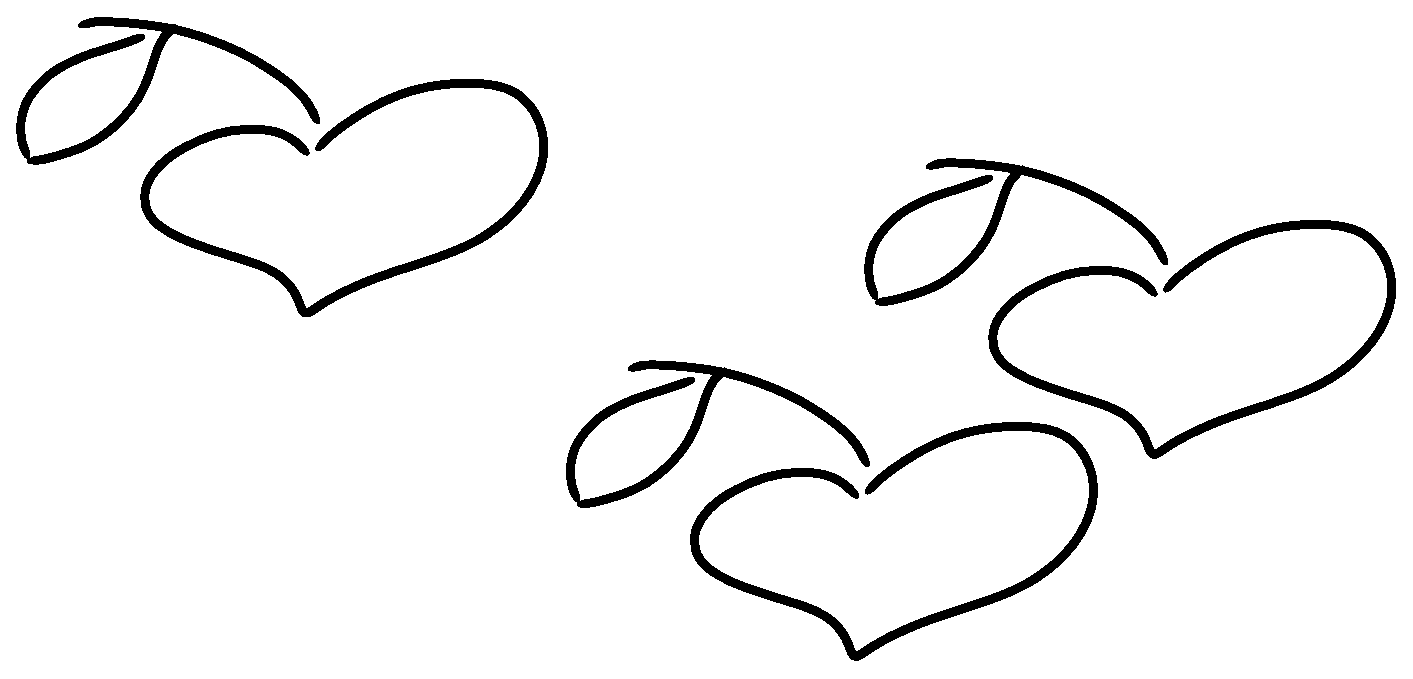
\includegraphics[width=0.6\linewidth]{images/Apples}
    %
    %\caption{
      %Одно яблоко, два яблока, ...~---~натуральные числа используются при счёте предметов.
    %}
    %\label{fig:naturals}
  %\end{figure}


  \subsection{Обратная функция}
  
  \begin{definition}
    Пусть есть функция~$f\colon X \hm\to Y$.
    
    \emph{Обратной} к ней называется функция $g\colon Y \hm\to X$, такая что
    \[
      \left\{\begin{aligned}
        &f\bigl(g(y)\bigr) = y,\quad \forall y \in Y\\
        &g\bigl(f(x)\bigr) = x,\quad \forall x \in X
      \end{aligned}\right.
    \]
    
    Обозначается обратная к~$f$ функция\footnote{
      Которая если есть, то единственная.
    } как $f^{-1}$.\footnote{
      Это не ``$f$ в степени минус один''~---~это одно неделимое обозначение.
    }
  \end{definition}
  
  \begin{proposition}[Существование обратной функции]
    Если функция~$f$ определена, строго монотонна и непрерывна на отрезке, то обратная функция также определена, строго монотонна и непрерывна на отрезке (другом).
  \end{proposition}
  
  \begin{proof}
    Пусть функция $f$ определена на отрезке $X \hm\equiv [a, b]$.
    Пусть для определённости функция $f$ монотонно возрастает, то есть $x_1 \hm< x_2 \hm\to f(x_1) \hm< f(x_2)$.
    
    Тогда, очевидно, $m \hm\equiv f(a)$ есть минимум $f\bigl([a, b]\bigr)$ (минимум множества значений функции~$f$ на отрезке $[a, b]$), а $M \hm\equiv f(b)$ есть максимум $f$ на $[a, b]$.
    По теореме о промежуточных значениях непрерывной на отрезке функции, образ отрезка $[a, b]$ под действием~$f$ есть отрезок $Y \hm\equiv [m, M]$.
    
    Покажем, что непрерывная для~$f$ функция существует.
    Пусть $y \hm\in Y$.
    Тогда найдётся $x \hm\in X$, такой что $f(x) \hm= y$.
    Но будет ли этот $x$ \emph{единственным}?
    (Можно ли построить \emph{правило} перевода из $Y$ в $X$?)
    Да, потому что~$f$ строго монотонна: если $x' \hm{\not=} x$, то либо $f(x') \hm< f(x)$ (при $x' \hm< x$), либо $f(x') > f(x)$ (при $x' \hm> x$), но в любом случае $f(x') \hm{\not=} f(x)$.
    То есть не существует $x' \hm{\not=} x$, такого чтоб было $f(x') \hm= f(x)$.
    Итого, правило однозначного перевода из $Y$ в $X$ существует, то есть существует обратная функция~$f^{-1}$.
    
    \begin{figure}[ht]
      \centering
      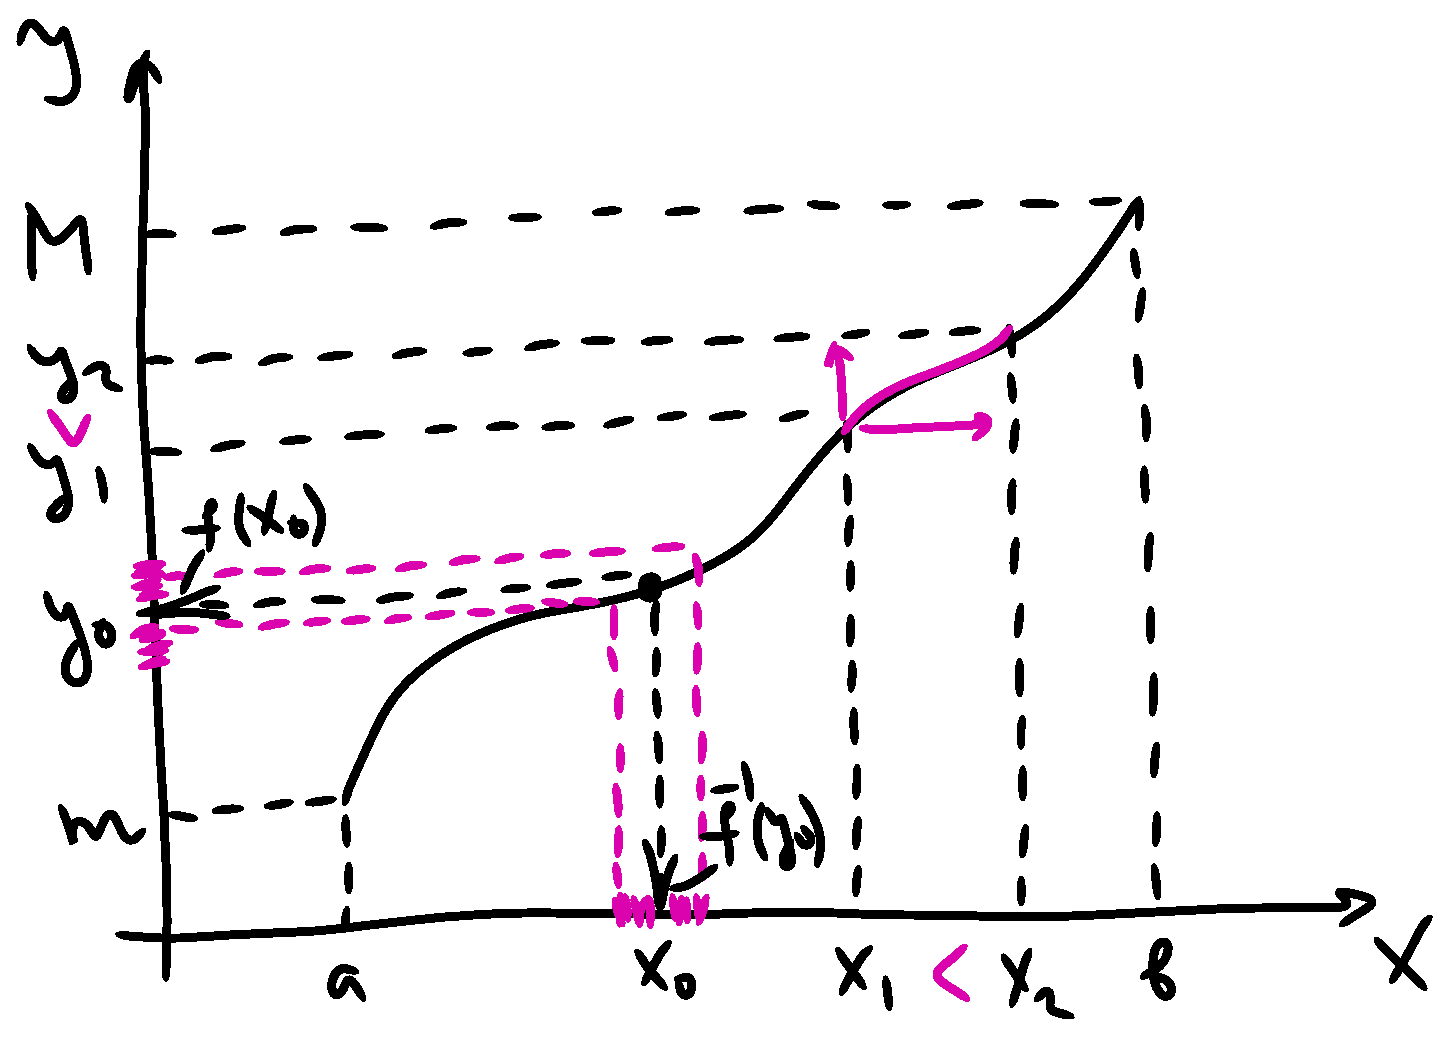
\includegraphics[width=0.6\linewidth]{images/ff-1}
    
      \caption{
        Строго монотонная непрерывная на отрезке функция~$f$ (и обратная для неё~$f^{-1}$, если смотреть на график под другим углом).
      }
      \label{fig:ff-1}
    \end{figure}
    
    Покажем, что обратная функция~$f^{-1}$ строго монотонна~(\ref{fig:ff-1}).
    (При этом из графика видно, что она должна строго монотонно возрастать.)
    Надо показать, что $y_1 \hm< y_2 \hm\to f^{-1}(y_1) \hm< f^{-1}(y_2)$.
    Но тогда можно просто воспользоваться монотонностью~$f$: если $y_1 \hm= f(x_1)$ и $y_2 \hm= f(x_2)$, то из неравенства для образов $y_1 \hm< y_2$ сразу получаем аналогичное неравенство для прообразов $x_1 \hm< x_2$.
    Потому что строгая монотонность~$f$ может по сути выражаться таким условием \emph{в две стороны}:
    \[
      x_1 < x_2 \quad\Leftrightarrow\quad f(x_1) < f(x_2)
    \]
    (определение монотонной~---~это только ``$\Rightarrow$'', но ``$\Leftarrow$'' в таком случае также будет верна.)
    
    Итак, осталось показать только непрерывность $f^{-1}$~(\ref{fig:ff-1}).
    Что есть непрерывность?
    ``Близость там~---~близость тут''.
    Но так как $f^{-1}$ есть по сути ``взгляд с другой стороны'' на отношение между $X$ и $Y$, налагаемое~$f$, то и ``взаимная близость'' (непрерывность) должна сохраниться.
    То есть план такой, чтоб показать непрерывность~$f^{-1}$, сведя всё к уже известной~$f$ (в принципе, как и в прошлом рассуждении про монотонность).
    
    Итак, $f$ непрерывна, значит, для любой последовательности $\{x_n\}\colon \lim_{n \to\infty} x_n \hm= x_0$ получим также $\lim_{n\to \infty} f(x_n) \hm= f(x_0)$ (где $x_0$~---~любая фиксированная точка~$X$).
    Аналогично, обратная $f^{-1}$ будет непрерывной, если для любой последовательности $\{y_n\}\colon \lim_{n \to\infty} y_n \hm= y_0$ получим также $\lim_{n\to \infty} \underbrace{f^{-1}(y_n)}_{x_n} \hm= f^{-1}(y_0) \hm\equiv x_0$ (где $y_0$~---~любая фиксированная точка~$Y$).
    Это надо доказать.
    Как вариант, допустим, что это не так, то есть что верно противное:
    \[
      \exists \{y_n\}\colon \lim_{n \to\infty} y_n \hm= y_0,\ \neg \left(\lim_{n\to \infty} f^{-1}(y_n) \hm= f^{-1}(y_0)\right)
    \]
    
    Факт того, что предел $\left\{f^{-1}(y_n)\right\}$ не есть $f^{-1}(y_0)$, перепишем в терминах окрестностей:
    \[
      \exists \{y_n\}\colon \lim_{n \to\infty} y_n \hm= y_0,\
        \exists \eps > 0\colon \forall N\ \exists n \geq N\colon \left|f^{-1}(y_n) - f^{-1}(y_0)\right| \geq \eps
    \]
    
    Иными словами, бесконечно много элементов $f^{-1}(y_n)$ последовательности $\left\{f^{-1}(y_n)\right\}$ лежат от $f^{-1}(y_0)$ на расстоянии $\eps$ и больше.
    Выделим их в отдельную подпоследовательность $\left\{f^{-1}\left(y_{n_k}\right)\right\} \hm= \left\{x_{n_k}\right\}$ (все элементы этой подпоследовательности находятся вне ``$\eps$-трубки'' от $f^{-1}(y_0) \hm= x_0$).
    Эта подпоследовательность лежит на отрезке $X \hm= [a, b]$, то есть ограничена, поэтому... из неё можно выделить сходящуюся подпоследовательность! (по теореме Больцано~--~Вейерштрасса)
    Обозначим её как $\left\{f^{-1}\left(y_{n_{k_l}}\right)\right\} \hm= \left\{x_{n_{k_l}}\right\}$.\footnote{
      Уже поздно останавливаться с усложнением обозначений.
      На самом деле у автора появился даже интерес всё корректно до конца описать, и посмотреть, насколько громоздкое обозначение в итоге получится)
    }
    Она сходится к чему-то из того же отрезка $X$,\footnote{
      Почему не может сходиться к чему-то вне отрезка?
    }
    при этом, очевидно, её предел отличен от $x_0$, и пусть равен $x_0'$.
    Но на этом уже ``всё'', потому что тогда в силу непрерывности и строгой монотонности~$f$ получаем:
    \[
      x_{n_{k_l}} \xrightarrow{l \to \infty} x_0' \not= x_0
        \quad\Rightarrow\quad f\bigl(x_{n_{k_l}}\bigr) \xrightarrow{l \to \infty} f(x_0') \not= f(x_0)
    \]
    
    Но ведь начали с того, что
    \[
      y_n \xrightarrow{n \to\infty} y_0
        \quad\Leftrightarrow\quad f\bigl(x_{n}\bigr) \xrightarrow{n \to \infty} f(x_0)
        \quad\Rightarrow\quad f\bigl(x_{n_{k_l}}\bigr) \xrightarrow{l \to \infty} f(x_0)
    \]
    
    Противоречие.
    Значит, предположение было неверно и обратная функция~$f^{-1}$ также непрерывна.
  \end{proof}

  
  
  \subsection{Отображение. Инъективность и сюръективность}
  
  {
    \small
    \emph{Источник раздела: \href{https://github.com/Alvant/GeomeSeminare/tree/master2022/seminars/linalge/seminar05}{ЛА5}.}
  }
  
  Об \emph{отображении} $\phi\colon X \hm\to Y$ можно думать как о правиле, которое \emph{каждому} элементу множества $X$ ставит в соответствие \emph{единственный} элемент множества $Y$\footnote{Множество $X$ в таком случае называется \emph{областью определения} отображения $\phi$ (множество ``допустимых'' входов). Таким образом, область определения~---~это часть определения отображения (определение области определения отображения~---~``тот самый $X$'' из определения отображения). Поэтому, когда в ``школьных'' номерах по математике просили ``найти область определения функции'', то имели в виду найти ``максимально возможное по количеству элементов множество, которое могло бы выступать в роли области определения функции'' (если бы привели полноценное определение этой функции, а не просто формулу).}~(\ref{fig:function}).
  Если отображение $\phi$ переводит элемент $x \hm\in X$ в элемент $y \hm\in Y$, то можно записать $\phi(x) \hm= y$, при этом $y$ называется \emph{образом} $x$, а $x$~---~прообразом $y$ (одним из возможных, если их несколько).
  
  \begin{figure}[h]
    \centering
  
    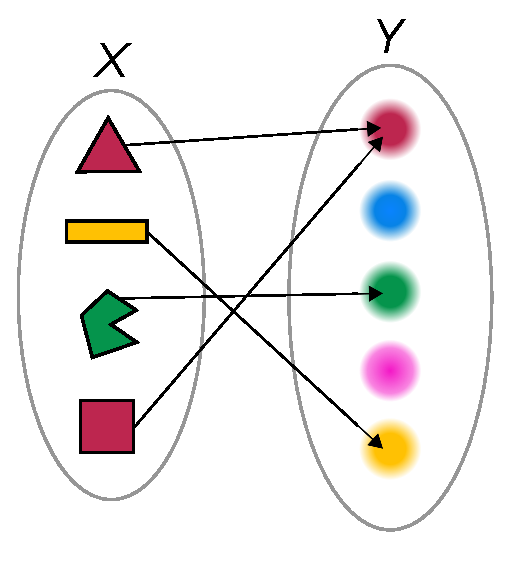
\includegraphics[width=0.3\columnwidth]{function}
  
    \caption{
      Отображение: каждому элементу $X$ соответствует единственный элемент $Y$.
      ({\small \href{https://en.wikipedia.org/wiki/Function\_(mathematics)\#/media/File:Function_color_example_3.svg}{Источник картинки}.})
    }
    \label{fig:function}
  \end{figure}
  
  % Про область определения:
  % https://math.stackexchange.com/a/2912118/451127
  % https://math.stackexchange.com/questions/63043/finding-a-functions-domain-from-the-functions-formula/63048#63048
  
  Можно отметить несколько свойств, которыми могут обладать произвольные отображения.
  
  \begin{definition}
    Отображение~$\phi$ называется \emph{инъективным}, если разные элементы отображаются в разные~(\ref{fig:injection}):
    $
      x_1, x_2 \hm\in X,\ x_1 \hm{\not=} x_2 \hm\Rightarrow \phi(x_1) \hm{\not=} \phi(x_2)
    $.
    Иными словами, если у элемента $y \hm\in Y$ есть прообраз, то он единственный.
  \end{definition}
  
  \begin{definition}
    Отображение~$\phi$ называется \emph{сюръективным}, если у \emph{любого} элемента $y \hm\in Y$ есть прообраз~(\ref{fig:surjection}):
    $
      \forall y \in Y\ \exists x \in X\colon \phi(x) = y
    $.
  \end{definition}
  
  \begin{figure}[ht]
    \centering
    
    \begin{subfigure}[b]{0.3\textwidth}
      \centering
    
      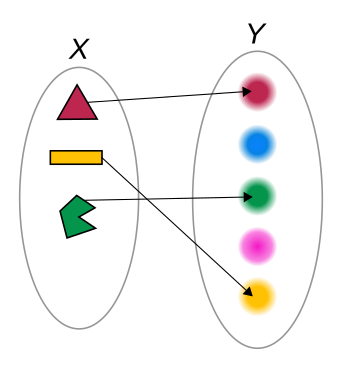
\includegraphics[width=\columnwidth]{injection}
    
      \caption{Инъекция.}
      \label{fig:injection}
    \end{subfigure}
    \hspace{2em}
    \begin{subfigure}[b]{0.3\textwidth}
      
      \centering
      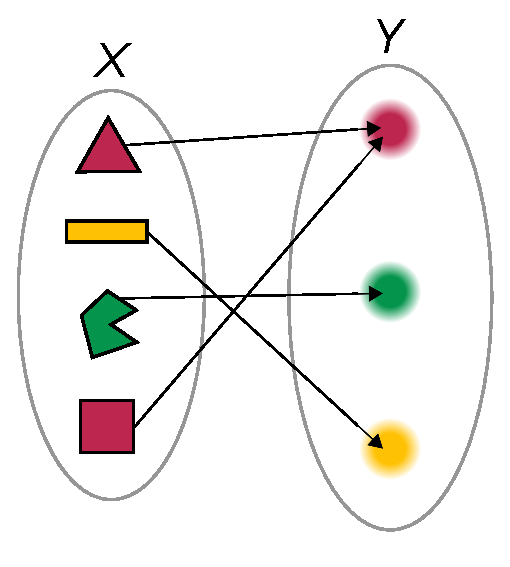
\includegraphics[width=\columnwidth]{surjection}
  
      \caption{Сюръекция.}
      \label{fig:surjection}
    \end{subfigure}
    
    \caption{Инъекция: ``разные в разные'', или ``если есть прообраз, то один''. Сюръекция: ``у~каждого есть хотя бы один прообраз''.}
  \end{figure}
  
  Факт наличия у отображения обоих приведённых выше свойств сразу выделяется в отдельное свойство.
  
  \begin{definition}
    Отображение~$\phi$ называется \emph{биективным}, если у \emph{любого} элемента $y \hm\in Y$ есть \emph{единственный} прообраз:
    $
      \forall y \in Y\ \exists ! x \in X\colon \phi(x) = y
    $.
  \end{definition}
  
  Помимо множества $X$ (области определения отображения $\phi$, или domain), и множества $Y$ (для которого, похоже, в русском языке нет специального названия, а по-английски~---~codomain) можно выделить ещё одно ``интересное'' множество, связанное с отображением~$\phi$~--- это \emph{множество значений} отображения $\Imag \phi \hm\subseteq Y$, которое определяется как совокупность всех элементов $y \hm\in Y$, в которые в принципе ``можно попасть'' под действием отображения:
  \[
    \Imag \phi = \{y \in Y \mid \exists x \in X\colon \phi(x) = y\}
  \]
  
  Тогда сюръективность означает, что $\Imag \phi \hm= Y$.
  
  
  
  
  
  \section{Дифференциал}

  % [X] определение дифференциала
  % []   + картинка
  % [X] дифференцируемость
  % [X] свойства дифференциала (сумма и т.п.)
  % [X] про историю определения производной

  \begin{figure}[ht]
      \centering
      
      \includegraphics[width=0.8\linewidth]{images/diff-f-df}
      
      \caption{Вблизи точки $x_0$ значение функции $f(x) \hm\approx f(x_0) \hm+ f'(x_0) \cdot (x - x_0)$.}
      \label{fig:diff-f}
  \end{figure}

  В ``близкой'' окрестности точки $x_0$ график функции ``в некотором приближении'' представим как график касательной в точке~$x_0$~(\ref{fig:diff-f}),~---~чем ближе окрестность, тем точнее такое представление~---~то есть приращение $\Delta f(x_0) \hm= f(x) \hm- f(x_0)$ в точке~$x_0$ функции можно ``оценить'' так:
  \[
    f(x) - f(x_0) \approx f'(x_0) \cdot (x - x_0)
  \]

  Оказывается, что можно написать и ``нормальное'' (строгое) равенство без приближений:
  \[
    f(x) - f(x_0) = f'(x_0) \cdot (x - x_0) + o(x - x_0),\quad x \to x_0
  \]
  где $o(x - x_0)$ есть $o$-малая от $x \hm- x_0$, то есть некоторая функция $g(x)$, для которой верно, что $\lim_{x \to x_0} \frac{g(x)}{x - x_0} \hm= 0$.
  (Поправка, отвечающая за ``точность'' приближения приращения функции как линейной функции от приращения аргумента~---~чем ближе к~$x_0$, тем точнее.)
  % (Таким образом, строчка выше~---~не совсем равенство в привычном смысле, это как бы ``равенство в пределе''.)
  Итого, для значения~$f(x)$ функции в некоторой точке~$x$ можно записать:
  \[
    f(x) = f(x_0) + f'(x_0) \cdot (x - x_0) + o(x - x_0),\quad x \to x_0
  \]

  Из этого соотношения возникают два понятия.
  
  \emph{Дифференциалом независимой переменной} называется её приращение:
  \[
    \diff x = \Delta x = x - x_0
  \]

  \emph{Дифференциалом функции} в точке~$x_0$ называется линейная по $\diff x$ часть приращения функции в этой точке (линейное ``приближение'' приращения функции):
  \begin{equation}\label{eq:diff-f}
    \diff f(x_0) = f'(x_0) \diff x   % f'(x_0) (x - x_0) = 
  \end{equation}

  % Тогда значение функции в точке~$x$ можно записать с помощью дифференциалов:
  % \[
  %   f(x) = f(x_0) + \underbrace{f'(x_0) \diff x}_{\diff f(x_0)} + o(x - x_0),\quad x \to x_0
  % \]

  А \emph{дифференцированием} называется процесс взятия производной функции.
  При этом получение дифференциала~\eqref{eq:diff-f} по сути тоже сводится к взятию производной.
  И правила дифференцирования функций во многом повторяют соответствующие правила для производных.
  Например, дифференциал константы $c \hm\in \RR$ равен нулю $\diff c \hm= 0$.
  Дифференциал суммы равен сумме дифференциалов.
  Константу как множитель можно выносить за знак дифференциала.
  Дифференциал произведения (распишем его подробнее):
  \[
    \diff (fg) = \diff f \cdot g + f \cdot \diff g
  \]
  так как, с одной стороны:
  \[
    \diff (fg) = (fg)' \diff x = (f'g + fg') \diff x
  \]
  и, с другой стороны:
  \[
    \diff f \cdot g + f \cdot \diff g = f' \diff x \cdot g + f \cdot g' \diff x
      = (f' g + fg') \diff x
  \]
  

  \subsection{``История''}

  Приведём краткий пересказ ``истории развития'' понятия производной.
  (Который кажется небесполезным для некоторого прояснения понятия дифференциала и его связи с производной.)
  
  \href{https://math.stackexchange.com/a/21209/451127}{Исторически} производная первоначально определялась как отношение ``бесконечно малых приращений'' $\frac{\diff y}{\diff x}$.
  То есть дробь $\frac{\diff y}{\diff x}$ в самом деле была дробью, в буквальном смысле.
  Но в связи с тем, что с ``бесконечно малым приращением'' есть некоторые проблемы (насколько бесконечно малое?), понятие производной в итоге пережило ``переосмысление''.
  Было предложено новое определение, через предел (то определение, которым и пользовались ранее).
  Таким образом, производная перестала быть отношением~---~она стала \emph{пределом} отношения.
  Но \emph{обозначение} $\frac{\diff y}{\diff x}$ сохранилось~---~и теперь оно обозначало не отношение ``бесконечно малых'', а просто производную, на это надо было смотреть не как на отношение чего-то, а как на один \emph{неделимый символ}.
  % (То же самое и с $\diff^2 y \hm/ \diff x^2$~---~на это можно смотреть не как на отношение, а как на цельный символ, обозначающий вторую производную.)
  Однако... после производной (выше в конспекте) было введено понятие дифференциалов $\diff x$ и $\diff y$.
  И получили, что производная $\frac{\diff y}{\diff x}$ (неделимый символ) равна отношению дифференциалов $\frac{\diff y}{\diff x}$ (а это уже просто дробь).
  % (Чем мы по сути и пользовались, когда, например, считали производную параметрически заданной функции, когда сверху и снизу делили на dt.)
  Таким образом, выражение $\frac{\diff y}{\diff x}$ может восприниматься двояко: либо как производная, либо как отношение дифференциалов (но не как отношение ``бесконечно малых'' приращений).
  % И в задаче, которую мы решали, судя по ответам, под d2y/dx2 имелась в виду именно вторая производная (хотя, не глядя на ответ, безошибочно угадать трактовку условия было бы нельзя).
  % Как-то так)
  % Такое вот объяснение.


  \subsection{С1, \S 13, \textnumero 179(3)} % или 179(3)? (не как в ДЗ)

  Исследовать на дифференцируемость функцию:
  \[
    % y = |sin x|
    y = x |x|
  \]

  \begin{solution}
    \begin{figure}[ht]
        \centering
        
        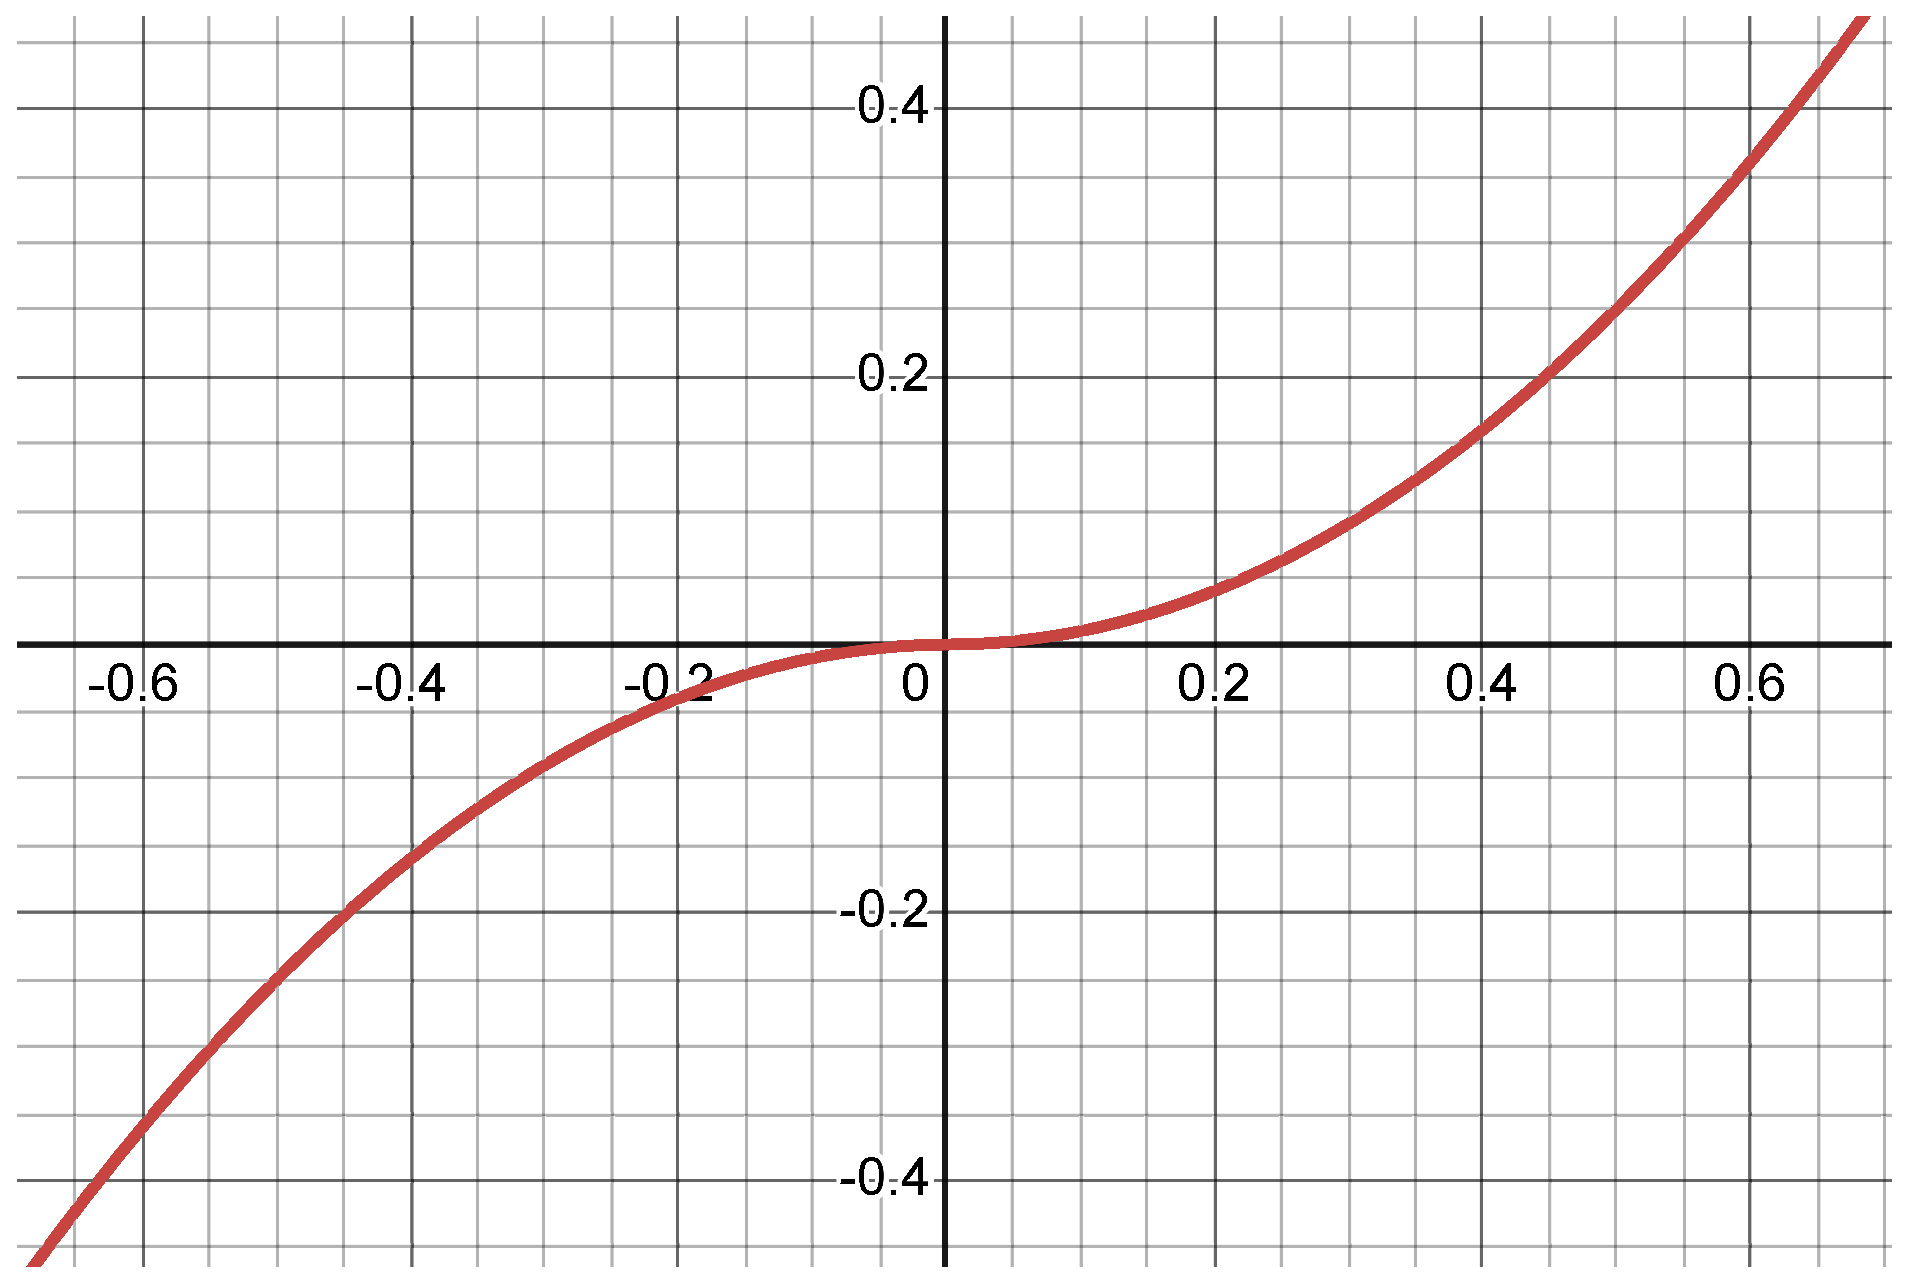
\includegraphics[width=0.8\linewidth]{images/x-mod-x}
        
        \caption{График функции $y \hm= x|x|$.}
        \label{fig:1-13-179(3)}
    \end{figure}

    Перепишем функцию в таком виде (без модуля):
    \[
      % y = \left\{
      %   \begin{aligned}
      %     &\hphantom{+}\sin x, & &\sin x \geq 0\\
      %     &-\sin x, & &\sin x < 0
      %   \end{aligned}
      % \right.
      y = \left\{
        \begin{aligned}
          &\hphantom{+}x^2, & &x \geq 0\\
          &{-}x^2, & &x < 0
        \end{aligned}
      \right.
    \]

    При рассмотрении функции на промежутках $(0, +\infty)$ и $(-\infty, 0)$ вопросов с производной нет~---~она получается просто из формулы, задающей функцию, по правилам взятия производной (на графике~(\ref{fig:1-13-179(3)}) это тоже видно):
    \[
      y' = \left\{
        \begin{aligned}
          &\hphantom{+}2x, & &x > 0\\
          &{-}2x, & &x < 0
        \end{aligned}
      \right.
    \]

    Отдельно стоит разобраться только с ``граничной'' точкой $x \hm= 0$ (граничной~---~в смысле на границах промежутков, где функция задаётся разными ``нормальными'' формулами).
    Попробуем найти производную в нуле по определению:
    \[
      f'(0) = \lim_{x \to 0} \frac{f(x) - f(0)}{x - 0}
        = \lim_{x \to 0} \frac{x |x|}{x}
        = \lim_{x \to 0} |x|
        = 0
    \]

    % TODO:
    % Можно бы было пойти по-другому.
    % Найдём \emph{пределы производных} слева и справа от интересуемой точки:
    % \[
    % \]

    Таким образом, функция дифференцируема на всей области определения ($\RR$), и производная находится по формуле:
    \[
      y' = 2|x|
    \]
  \end{solution}


  \subsection{С1, \S 13, \textnumero 197(3)}

  Найти производную обратной к~$f$ функции в указанной точке:
  \begin{equation}\label{eq:1-13-197(3)}
    y = \underbrace{0{.}1x + e^{0{.}1 x}}_{f(x)},\quad y = 1
  \end{equation}

  \begin{solution}
    % определение обратной функции
    % вывод производной обратной функции

    Если есть функция $f\colon X \hm\to Y$, то \emph{обратной} к ней называется функция $g\colon Y \hm\to X$, такая что:
    \[
      \left\{
        \begin{aligned}
          &g\bigl(f(x)\bigr) = x,\quad \forall x \in X\\
          &f\bigl(g(y)\bigr) = y,\quad \forall y \in Y
        \end{aligned}
      \right.
    \]

    Обратная к $f$ функция обычно обозначается как $f^{-1}$ (это одно неделимое обозначение, а не ``$f$ в степени'').

    Дифференцируя по $x$ первое уравнение системы, получаем:
    \[
      \begin{aligned}
        &g'\bigl(f(x)\bigr) = x'\\
        &g'(y)|_{y = f(x)} \cdot f'(x) = 1
      \end{aligned}
    \]

    Таким образом,
    \[
      \boxed{g'(y) = \left.\frac{1}{f'(x)}\right|_{x = g(y)}}
    \]

    Получить связь между производными прямой и обратной функций можно бы было и из связи между производной и дифференциалами:
    \[
      \left.\begin{aligned}
        &f'(x) = \frac{\diff y}{\diff x}\\
        &g'(y) = \frac{\diff x}{\diff y}
      \end{aligned}\ \right|
      \Rightarrow g'(y) = \frac{1}{\diff y /\!\diff x}
        = \frac{1}{f'(x)}
    \]

    Возвращаясь к функции из номера~\eqref{eq:1-13-197(3)}, найдём сначала тот $x$, который соответствует $y \hm= 1$ (точке, где просят посчитать производную обратной функции):
    \[
      1 = 0{.}1x + e^{0{.}1 x} \Leftrightarrow x = 0
    \]

    Производная исходной функции:
    \[
      \begin{aligned}
        &y' = 0{.}1 + 0{.}1 \cdot e^{0{.}1 x}\\
        &y'(0) = 0{.}2
      \end{aligned}
    \]

    Тогда производная обратной функции:
    \[
      \begin{aligned}
        &(f^{-1})' = \frac{1}{0{.}1 + 0{.}1 \cdot e^{0{.}1 x}}\\
        &(f^{-1})'(1) = 5
      \end{aligned}
    \]
  \end{solution}


  \subsection{С1, \S 13, \textnumero 201(4)}
  % TODO: 201(3) -- можно только нарисовать (номер из ДЗ)

  Найти $f'(x)$ для функции $y \hm= f(x)$, заданной параметрически:
  \begin{equation}\label{eq:1-13-204(1)-given}
    \left\{
      \begin{aligned}
        &x = x(t) = a \ch t\\
        &y = y(t) = b \sh t
      \end{aligned}
    \right.,\quad -\infty < t < 0
  \end{equation}

  % 201(3)
  % \[
  %   \left\{
  %     \begin{aligned}
  %       &x = a \cos t\\
  %       &y = b \sin t
  %     \end{aligned}
  %   \right.,\quad 0 < t < \pi
  % \]

  \begin{remark}    
    Скажем пару слов про упоминаемые в задаче гиперболические функции.

    Гиперболический косинус (``чосинус''):
    \[
      \ch x = \frac{e^x + e^{-x}}{2}
    \]
    
    Гиперболический синус (``шинус''):
    \[
      \sh x = \frac{e^x - e^{-x}}{2}
    \]

    %\begin{figure}
      %\centering
    %
      %\begin{subfigure}[b]{0.4\textwidth}
        %\centering
        %
        %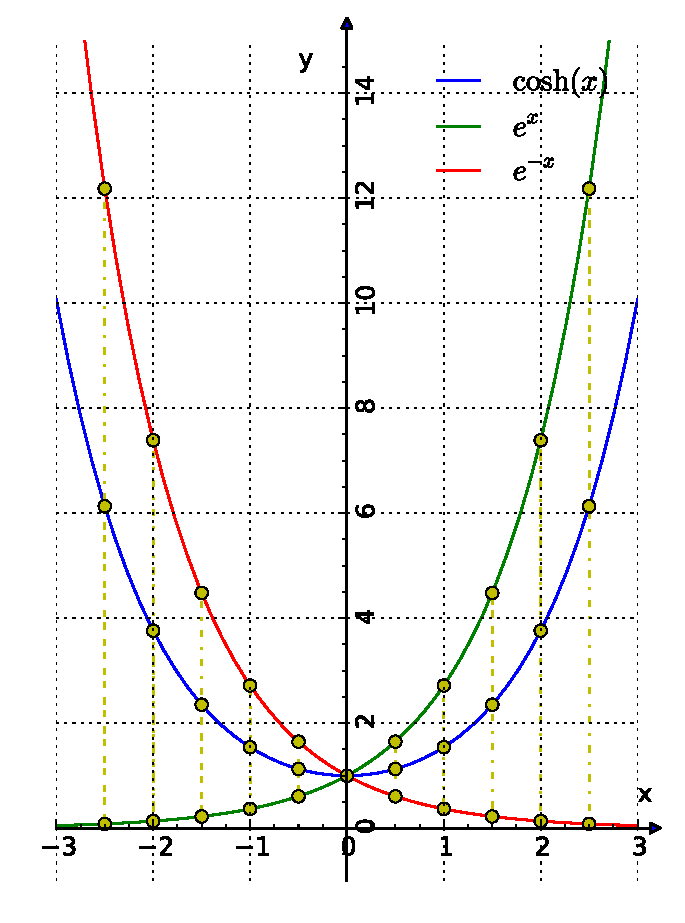
\includegraphics[width=\textwidth]{images/ch-x}  % TODO: eps
        %
        %\caption{
          %График функции $y = \ch x$.
          %({\small \href{https://commons.wikimedia.org/wiki/File:Hyperbolic_and_exponential;_cosh.svg}{Источник}})
        %}
        %\label{fig:ch-x}
      %\end{subfigure}
      %%
      %\hfill
      %%
      %\begin{subfigure}[b]{0.4\textwidth}
        %\centering
        %
        %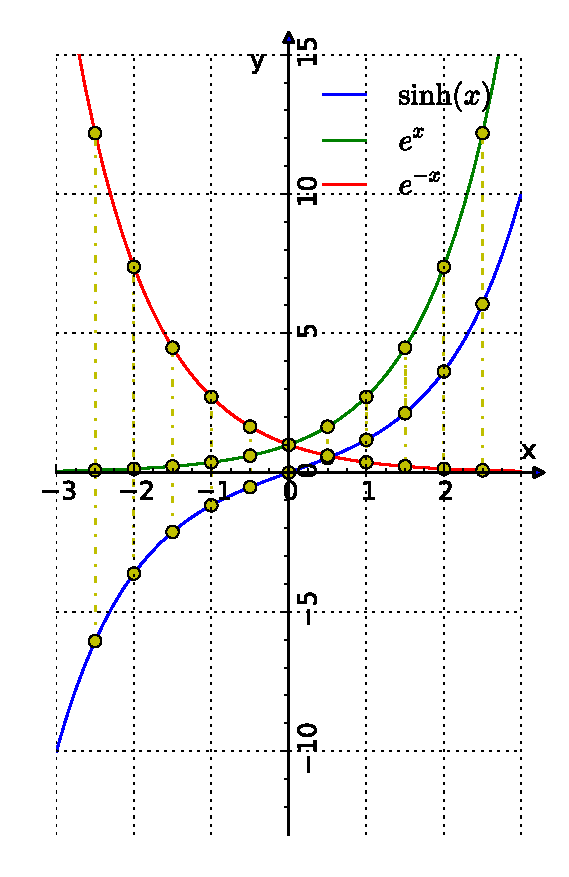
\includegraphics[width=\textwidth]{images/sh-x}  % TODO: eps
        %
        %\caption{
          %График функции $y = \sh x$.
          %({\small \href{https://commons.wikimedia.org/wiki/File:Hyperbolic_and_exponential;_sinh.svg}{Источник}})
        %}
        %\label{fig:sh-x}
      %\end{subfigure}
    %
      %\caption{
        %Графики ``чосинуса'' и ``шинуса''.
      %}
      %\label{fig:ch-x-sh-x}
    %\end{figure}
    
    \begin{figure}
      \centering
    
      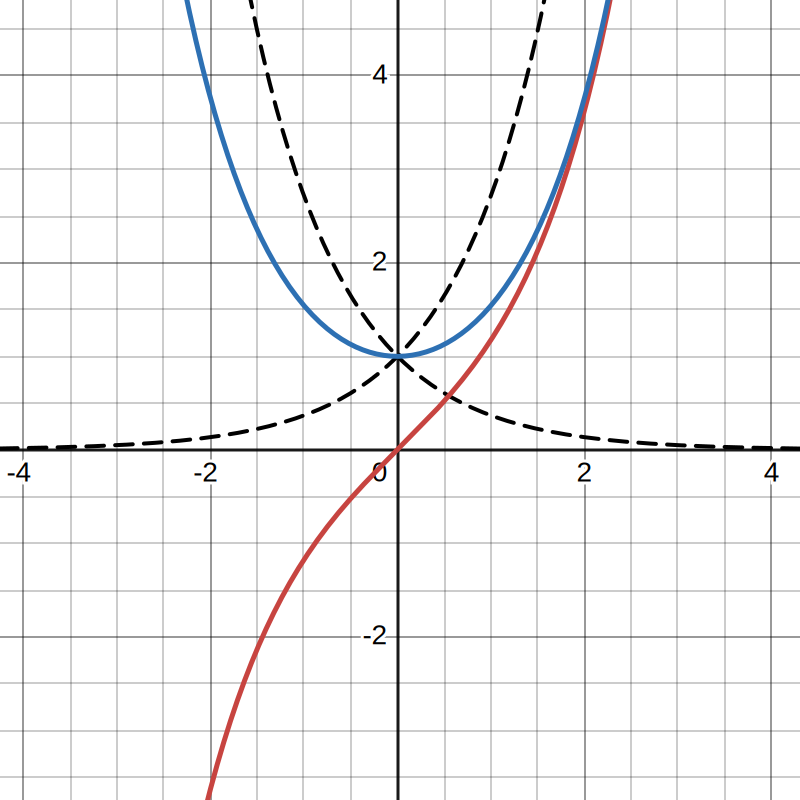
\includegraphics[width=0.5\textwidth]{images/ch-x-sh-x}
    
      \caption{
        Графики ``\href{https://commons.wikimedia.org/wiki/File:Hyperbolic_and_exponential;_cosh.svg}{чосинуса}'' (синий) и ``\href{https://commons.wikimedia.org/wiki/File:Hyperbolic_and_exponential;_sinh.svg}{шинуса}'' (красный).
        Пунктиром приведены графики функций $y \hm= e^x$ и $y \hm= e^{-x}$.
      }
      \label{fig:ch-x-sh-x}
    \end{figure}

    Кажется, что понять, что это вообще такое, лучше помогают графики~(\ref{fig:ch-x-sh-x}).

    Так, например, видно, что:
    \[
      \begin{aligned}
        &\ch 0 = 1\\
        &\sh 0 = 0
      \end{aligned}
    \]

    Очевидно, что $\ch x \hm> \sh$.
    Но, кроме этого, можно заметить, что:
    \[
      \sh x \sim \ch x,\quad x \to +\infty
    \]

    Также из графиков можно увидеть, что $\ch x$~---~это выпуклая вверх функция (``чашка''), а $\sh x$ меняет выпуклость в нуле: с выпуклой вниз (вогнутой~---~``колокол''), на выпуклую вверх.

    Ещё из свойств можно отметить: чётность у $\ch x$:
    \[
      \ch x = \ch{-x}
    \]
    и нечётность у $\sh x$:
    \[
      \sh x = {-}\sh{-x}
    \]

    Соотношение же, которого из графиков уже не видно:
    \[
      \ch^2 x - \sh^2 x = 1
    \]

    Но можно проверить, просто подставив в формулу выражения, которыми определяются $\ch x$ и $\sh x$:
    \[
      \ch^2 x - \sh^2 x = 
        \left(\frac{e^x + e^{-x}}{2}\right)^2 - \left(\frac{e^x - e^{-x}}{2}\right)^2 = 1
    \]

    Производные:
    \[
      \begin{aligned}
        &\ch'x = \left(\frac{e^x + e^{-x}}{2}\right)' = \sh x\\
        &\sh'x = \left(\frac{e^x - e^{-x}}{2}\right)' = \ch x
      \end{aligned}
    \]
  \end{remark}
  
  \begin{solution}
    Параметрически заданная функция~---~построить её график (в осях $X$ и $Y$) можно по точкам, перебирая значения $t$ из заданного промежутка: $\{t_1, t_2, \ldots, t_n\}$, и вычисляя по ним через функции $x(t)$ и $y(t)$ координаты: $\Bigl\{\bigl(x(t_1), y(t_1)\bigr), \bigl(x(t_2), y(t_2)\bigr), \ldots\Bigr\}$.

    В данном же случае можно получить зависимость $y \hm= f(x)$ и в явном виде.
    Так как $t \hm< 0$, то $\sh t \hm< 0$, поэтому:
    \begin{equation}\label{eq:1-13-204(1)-nonparametric}
      y = b \sh t = b \cdot \left(-\sqrt{\ch^2 t - 1}\right)
        = -b \sqrt{\left(\frac{x}{a}\right)^2 - 1}
    \end{equation}

    Но вернёмся к параметрическому заданию функции...
    Производную такой функции можно найти как:
    \[
      f'(x) = \frac{\diff y}{\diff x}
        = \frac{\diff y / \!\diff t}{\diff x / \!\diff t}
        = \frac{y'_t}{x'_t}
    \]

    Поэтому для функции из задачи:
    \begin{equation}\label{eq:1-13-204(1)}
        f'(x) = \frac{b \ch t}{a \sh t}
    \end{equation}
    
    Производная~$f'(x)$~---~функция от $x$, но выражение в~\eqref{eq:1-13-204(1)} справа~---~это функция от $t$...
    Понимать запись стоит в том смысле, что значение производной в точке $x$ считается с помощью~$t$, соответствующего этому самому~$x$.
    Но можно попробовать и выразить $f'$ через~$x$ в явном виде.
    Из~\eqref{eq:1-13-204(1)-given} имеем $\ch t \hm= x \hm/ a$.
    Что делать с $\sh t$?
    Так как по условию $t \hm< 0$, то $\sh t \hm< 0$, поэтому можно выразить его из тождества:
    \[
      \ch^2 t - \sh^2 t = 1 \xrightarrow{\sh t \hm< 0}
        \sh t = -\sqrt{\ch^2 t - 1} = -\sqrt{(x / a)^2 - 1}
    \]

    И итоговое выражение для $f'(x)$ в таком случае:
    \[
      f'(x) = -\frac{b}{a} \cdot \frac{x}{\sqrt{x^2 - a^2}}
    \]

    (Убеждаемся, что оно совпадает с производной, которую можно бы было посчитать по связи $y \hm= f(x)$, полученной в явном виде~\eqref{eq:1-13-204(1)-nonparametric}.)
  \end{solution}

  
  \subsection{С1, \S 13, \textnumero 214(1)}

  Найти дифференциал функции в указанной точке:
  \[
    d\left(\frac{1}{x} + \ln \frac{x - 1}{x}\right),\quad x = -1
  \]
  
  \begin{solution}
    Если есть функция
    \[
      y = f(x)
    \]
    то её дифференциал равен:
    \[
      \diff f(x) = f'(x) \diff x
    \]

    Имея в виду, что интересует дифференциал функции в точке $x \hm= -1$, можно немного упростить (с целью дальнейшего дифференцирования) выражение, которым определяется функция:
    \[
      f(x) = \frac{1}{x} + \ln \frac{x - 1}{x}
        = \frac{1}{x} + \ln{(1 - x)} - \ln{{-}x},\quad x < 0
    \]
    (хотя можно бы было и не упрощать логарифм~---~взятие производной было бы не сильно сложнее...)

    Поэтому дифференциал равен:
    \begin{equation*}
    \begin{split}
      \diff f(x) &= \diff \left(\frac{1}{x} + \ln \frac{x - 1}{x}\right)
        = \diff \left(\frac{1}{x} + \ln{(1 - x)} - \ln{-x}\right)\\
        &= -\frac{1}{x^2} \diff x + \frac{1}{1 - x} \cdot (-1) \diff x - \frac{1}{-x} \cdot (-1) \diff x
        = \left(-\frac{1}{x^2} + \frac{1}{x - 1} - \frac{1}{x}\right) \diff x
    \end{split}
    \end{equation*}

    В указанной точке:
    \[
      \diff f(x)|_{x = -1}
        = \left.\left(-\frac{1}{x^2} + \frac{1}{x - 1} - \frac{1}{x}\right)\right|_{x = -1} \diff x
        = -\frac{1}{2} \diff x
    \]
  \end{solution}

  
  \subsection{С1, \S 13, \textnumero 173}

  Дана функция $y = f(x)$:
  \[
    y = \left\{
      \begin{aligned}
        &|x|^{\alpha} \sin{\left(\frac{1}{x}\right)}, & &\mbox{если } x \not= 0\\
        &0, & &\mbox{если } x = 0
      \end{aligned}
    \right.
  \]
  
  При каких значениях $\alpha$ функция в точке $x \hm= 0$:
  \begin{enumerate}
    \item непрерывна
    \item имеет производную
    \item имеет непрерывную производную
  \end{enumerate}
  
  \begin{solution}
    \mbox{}\par\noindent  % https://latex.org/forum/viewtopic.php?t=23229
    \emph{Непрерывность}.
    Функция $f(x)$ непрерывна в точке $x_0$, если она определена в некоторой окрестности этой точки и если:
    \[
      \lim_{x \to x_0} f(x) = f(x_0)
    \]

    Стремление $x \to x_0$ означает приближение $x$ неограниченно близко к $x_0$.
    В задаче $x_0 \hm= 0$, а формула, которой функция определяется во всех точках, кроме нуля, включает модуль $|x|$~---~поэтому можно рассмотреть случаи приближения к нулю с каждой из сторон: слева и справа (тогда модуль можно будет раскрыть с определённым знаком).
    Например, рассмотрим предел при $x \hm\to x_0 \hm+ 0$ (то есть $x$ приближается к $x_0$ неограниченно близко, но всегда остаётся больше $x_0$):
    \[
      \lim_{x \to +0} f(x) \overset{\?}{=} f(0) = 0
    \]
    \[
      \lim_{x \to +0} f(x)
        = \lim_{x \to +0} x^{\alpha} \sin{\left(\frac{1}{x}\right)}
    \]

    Равенство этого предела нулю равносильно равенству нулю следующего предела:\footnote{
      Будем считать, что это ``очевидно'', хотя можно и более строго объяснить (при этом в одну сторону точно очевидно).
    }
    \[
      \lim_{x \to +0} x^{\alpha} = 0
    \]

    Когда это будет выполняться?
    Очевидно, подходят $\alpha \hm> 0$.
    При этом $\alpha \hm< 0$ не подходят (тогда в пределе будет бесконечность, а не ноль).
    При $\alpha \hm= 0$ в пределе будет единица.
    Таким образом:
    \[
      \lim_{x \to +0} f(x) = 0
        \quad\Leftrightarrow\quad \lim_{x \to +0} x^{\alpha} = 0
        \quad\Leftrightarrow\quad \alpha > 0
    \]

    С приближением к нулю слева $x \hm\to -0$ всё бы было аналогично (только появился бы знак ``минус'', который бы ни на что не повлиял).

    \medskip
    
    \noindent
    \emph{Наличие производной}.
    В нуле функция определяется ``по-особому'', поэтому посчитать в этой точке производную можно только по определению.\footnote{
      По крайней мере, автор конспекта другого способа не знает)
    }
    Итак, функция $f(x)$ имеет производную в точке~$x_0$, если существует предел:
    \[
      \lim_{x \to x_0} \frac{f(x) - f(x_0)}{x - x_0}
    \]
    (конечный либо ``плюс-минус-бесконечный'').\footnote{
      Но не ``просто бесконечный''.
    }

    Опять же, вместо ``просто'' стремления $x \hm\to 0$, можно начать с рассмотрения более простого (понятного в условиях задачи) случая стремления $x \hm\to 0$ с какой-нибудь одной стороны~---~то есть с поиска левой ($x \hm\to 0 \hm- 0$) или правой ($x \hm\to 0 \hm+ 0$) производной.
    Например, будем опять приближаться к нулю справа:
    \[
      \lim_{x \to +0} \frac{f(x) - f(0)}{x - 0}
        = \lim_{x \to +0} \frac{x^{\alpha} \sin{\left(\frac{1}{x}\right)}}{x}
        = \lim_{x \to +0} x^{\alpha - 1} \sin{\left(\frac{1}{x}\right)}
    \]

    Когда этот предел будет существовать?
    Из-за множителя с синусом снова остаётся единственная возможность: когда $x^{\alpha - 1} \hm{\xrightarrow{x \to +0}} 0$ (если этот предел будет определённого знака бесконечен, то производной справа из-за синуса всё равно никакой не будет).
    Таким образом:
    \[
      \exists f'_{+}(0) = \lim_{x \to +0} \frac{f(x) - f(0)}{x - 0}
        \quad\Leftrightarrow\quad \lim_{x \to +0} x^{\alpha - 1} = 0
        \quad\Leftrightarrow\quad \alpha > 1
    \]

    С приближением к нулю слева $x \hm\to -0$ всё бы было аналогично.
    То есть при $\alpha \hm> 1$ получили бы также:
    \[
      f'_{-}(0) = \lim_{x \to -0} \frac{f(x) - f(0)}{x - 0} = 0
    \]

    А из равенства односторонних производных следует и существование ``просто'' производной:
    \[
      f'(0) = f'_{+}(0) = f'_{-}(0) = 0
    \]
    (если приближаться к нулю попеременно с двух сторон, на каждой из которых в качестве производной получается ноль, то и в итоге будет ноль).

    \medskip
    
    \noindent
    \emph{Наличие непрерывной производной}.
    Производная $f'(x)$ функции $f(x)$ непрерывна в точке~$x_0$, если она определена в некоторой окрестности этой точки и если:
    \[
      \lim_{x \to x_0} f'(x) = f'(x_0)
    \]

    Надо искать предел производной.
    Поэтому получим сначала формулу, которой определяется $f'(x)$.

    Исходная функция:
    \[
      f(x) = \left\{
        \begin{aligned}
          &x^{\alpha} \sin{\left(\frac{1}{x}\right)}, & &x > 0\\
          &(-x)^{\alpha} \sin{\left(\frac{1}{x}\right)}, & &x < 0\\
          &0, & &x = 0
        \end{aligned}
      \right.
    \]

    Производная:
    \[
      f'(x) = \left\{
        \begin{aligned}
          &\alpha x^{\alpha - 1} \sin{\left(\frac{1}{x}\right)} + x^{\alpha} \cos{\left(\frac{1}{x}\right)} \left(-\frac{1}{x^2}\right), & &x > 0\\
          &\alpha (-x)^{\alpha - 1} \cdot (-1) \cdot \sin{\left(\frac{1}{x}\right)} + (-x)^{\alpha} \cos{\left(\frac{1}{x}\right)} \left(-\frac{1}{x^2}\right), & &x < 0\\
          &0, & &x = 0
        \end{aligned}
      \right.
    \]

    Рассмотрим сначала односторонний предел производной:
    \[
      \lim_{x \to +0} f'(x) \overset{\?}{=} f'(0)
    \]
    \[
      \lim_{x \to +0} \alpha x^{\alpha - 1} \sin{\left(\frac{1}{x}\right)} + x^{\alpha} \cos{\left(\frac{1}{x}\right)} \left(-\frac{1}{x^2}\right) \overset{\?}{=} 0
    \]
    \[
      \lim_{x \to +0} x^{\alpha - 2} \cdot \left\{
        \alpha x \sin{\left(\frac{1}{x}\right)} - \cos{\left(\frac{1}{x}\right)}
      \right\} \overset{\?}{=} 0
    \]

    Видно, что равенство этого предела нулю равносильно равенству нулю предела:
    \[
      \lim_{x \to +0} x^{\alpha - 2} = 0
    \]

    Что приводит к условию $\alpha \hm> 2$.

    С приближением к нулю слева $x \hm\to -0$ всё бы было аналогично.
    То есть при $\alpha \hm> 2$ получили бы также:
    \[
      \lim_{x \to -0} f'(x) = 0 = f'(0)
    \]

    Значит, и при ``просто'' стремлении к нулю (возможно, попеременно с двух сторон) получили бы в пределе $f'(0)$.

    \begin{remark}
      Из полученных условий на $\alpha$ видно, что свойства непрерывности функции в точке, наличия в этой точке производной и непрерывности производной в точке~---~упорядочены по ``силе'', от более слабых к более сильным.
      % Непрерывность включает в себя наличие производной, что в свою очередь включает непрерывность производной~(\ref{fig:function-circles}).  % После второго прочтения показалось, что странновато звучит (трактуется неоднозначно)
      Из непрерывности производной следует существование конечной производной, из чего в свою очередь следует непрерывность~(\ref{fig:function-circles}).\footnote{
        В определении производной  под пределом стоит дробь, в числителе которой находится разность $f(x) - f(x_0)$.
        Если она не стремится к нулю при стремлении $x$ к $x_0$, то предел не будет конечным.
      }

      \begin{figure}[ht]
          \centering
          
          \includegraphics[width=0.3\linewidth]{images/function-circles}
          
          \caption{Соотношения между непрерывными на промежутке функциями, дифференцируемыми и непрерывно дифференцируемыми.}  % TODO: промежуток -- ?
          \label{fig:function-circles}
      \end{figure}

      Совокупность всех функций, непрерывных на отрезке~$[a, b]$ (класс функций), может обозначаться как $C[a, b]$.
      Совокупность функций, дифференцируемых на отрезке~$[a, b]$, похоже, никак специальным образом не обозначается.\footnote{
        \href{https://math.stackexchange.com/questions/4450788/space-of-differentiable-functions\#comment9321095_4450788}{Не только автор конспекта так считает}.
      }
      Класс же непрерывно дифференцируемых на отрезке~$[a, b]$ функций есть $C^1[a, b]$.

      Таким образом, тот факт, что из непрерывной дифференцируемости функции на отрезке следует её непрерывность на этом отрезке, можно выразить таким образом:
      \[
        C^1[a, b] \subset C[a, b]
      \]
    \end{remark}
  \end{solution}


  \subsection{С1, \S 14, \textnumero 10(1)}

  Написать уравнение касательной и нормали к кривой в точке:
  \begin{equation}\label{eq:1-14-10(1)}
    x^3 + y^2 + 2x - 6 = 0,\quad (x_0, y_0) = (-1, 3)
  \end{equation}
  
  \begin{solution}
     \begin{figure}[ht]
         \centering
         
         \includegraphics[width=0.8\linewidth]{images/tangent-and-normal}
         
         \caption{Касательная и нормаль к графику кривой $F(x, y) \hm= 0$ в точке $(x_0, y_0)$.}
         \label{fig:tangent-and-normal}
     \end{figure}

     Заметим, что уравнением~\eqref{eq:1-14-10(1)} задаётся зависимость $y$ от $x$, но эта зависимость~---~не функция!
     (Например, одному ``икс'' $x \hm= 0$ удовлетворяют два ``игрека'' $y \hm= \pm \sqrt{6}$.)

     Проверим для начала на всякий случай, что точка в самом деле лежит на кривой:
     \[
       (-1)^3 + 3^2 + 2 \cdot (-1) - 6 = 0
     \]

     Уравнение касательной получается сразу из связи между производной функции в точке и её дифференциалом в этой точке:\footnote{
       Функции~---~по которой~$y$ определяется через $x$ хотя бы в некоторой окрестности точки $(x_0, y_0)$.
     }
     \[
       \diff f(x_0) = f'(x_0) \diff x
     \]

     Дифференциал в точке~---~это как линейное приближение приращения функции в точке $\Delta f(x_0) \hm= f(x) - f(x_0)$.
     Сам же дифференциал тоже по сути равен приращению, но не самой функции, а функции~$f_{\mbox{\scriptsize кас}}$, задающей касательную:
     \[
       \diff f(x_0) = f_{\mbox{\scriptsize кас}}(x) - f_{\mbox{\scriptsize кас}}(x_0)
     \]
     (при этом $f_{\mbox{\scriptsize кас}}(x_0) \hm= f(x_0)$)

     Дифференциал же независимой переменной $\diff x$ просто равен её приращению (относительно исходной точки~$x_0$):
     \[
       \diff x = \Delta x = x - x_0
     \]

     Объединяя вместе приведённые рассуждения, получаем уравнение касательной к функции $f$ в точке~$x_0$ в общем виде:
     \[
       f_{\mbox{\scriptsize кас}}(x) - f(x_0) = f'(x_0) \cdot (x - x_0)
     \]

     Чтобы выписать это уравнение для указанной кривой, не хватает производной~$f'(x_0)$.
     Но в явном виде зависимости $f(x)$ нет~---~функция задана неявно.
     Поэтому, например, продифференцируем обе части~\eqref{eq:1-14-10(1)}:
     \[
       3 x^2 \diff x + 2 y \diff y + 2 \diff x = 0
     \]

     Отсюда получаем:
     \[
       \frac{\diff y}{\diff x} =  \frac{-2 - 3 x^2}{2 y}
     \]

     В интересуемой точке $(x_0, y_0) = (-1, 3)$:
     \[
       \left.\frac{\diff y}{\diff x}\right|_{(x, y) = (x_0, y_0)}
         = \frac{-5}{6}
     \]
     А это и есть $f'(x_0)$.

     Поэтому для уравнения касательной получаем:
     \[
       f_{\mbox{\scriptsize кас}}(x) = f(x_0) + f'(x_0) \cdot (x - x_0)
         = 3 - \frac{5}{6} \cdot (x + 1)
     \]

     \medskip
     
     Нормаль к графику функции $f(x)$ в точке $x_0$ также проходит через $(x_0, y_0)$, но под углом $90$\degree к касательной~(\ref{fig:tangent-and-normal}).
     То есть если $\alpha$~---~угол наклона касательной (угол между касательной и положительным направлением оси $X$), то $\alpha \hm+ \frac{\pi}{2}$ будет углом наклона нормали:
     \[
       \begin{aligned}
         &\tg \alpha = f'(x_0) = \frac{-5}{6}\\
         &\tg{\left(\alpha + \frac{\pi}{2}\right)} = -\ctg \alpha = -\frac{1}{\tg \alpha} = \frac{6}{5}
       \end{aligned}
     \]

     Уравнение нормали:
     \[
       f_{\mbox{\scriptsize норм}}(x) = 3 + \frac{6}{5} \cdot (x + 1)
     \]
  \end{solution}


  \section{Производные и дифференциалы высших порядков}

  % [X] определение (рекурсивное)
  % [X] пример с cos(x)
  % [X] производная произведения
  % [X] пример с x^2 cos(x)
  % [X] дифференциал n-ой степени

  Производная~$f'(x)$ функции~$f(x)$~---~тоже функция.
  У которой тоже может быть производная.
  У которой тоже может быть производная.
  И так далее.
  Приходим к понятию производных порядка $n \hm\geq 2$:
  \[
    \begin{aligned}
      &f''(x) = (f')'(x)\\
      &f'''(x) = (f'')'(x)\\
      &\ldots\\
      &f^{(n)}(x) = \left(f^{(n - 1)}\right)'(x)
    \end{aligned}
  \]

  Если положить $f^{(0)}(x) \hm\equiv f(x)$, то можно привести такое рекурсивное определение производной:
  \[
    f^{(n)} = \left\{
      \begin{aligned}
        &f,              & &n = 0\\
        &\left(f^{(n - 1)}\right)', & &n \geq 1 
      \end{aligned}
    \right.
  \]

  \begin{example}\label{eq:cos-x}
    Найдём $n$-ую производную функции $\cos x$:
    \[
      \begin{aligned}
        &\cos' x = {-}\sin x\\
        &\cos'' x = ({-}\sin x)' = {-}\cos x\\
        &\cos''' x = ({-}\cos x)' = \sin x\\
        &\cos^{(4)} x = \sin' x = \cos x
        &\ldots
      \end{aligned}
    \]
    (после третьей производной, очевидно, процесс ``зацикливается''~---~опят получился $\cos x$).
    Можно заметить, что $\left|\cos^{(2k)}\right| \hm= |\cos x|$ и $\left|\cos^{(2k + 1)}\right| \hm= |\sin x|$, а знак ``как-то'' чередуется, итого $n$-ую производную можно описать формулой:
    \[
      \cos^{(n)}(x) = \left\{
        \begin{aligned}
          &(-1)^{n/2} \cos x, & &n = 2k,\ k = 0, 1, \ldots\\
          &(-1)^{(n + 1)/2} \sin x, & &n = 2k + 1,\ k = 0, 1, \ldots\\
        \end{aligned}
      \right.
    \]
  \end{example}

  Отдельно стоит отметить сюжет о вычислении $n$-ой производной произведения...
  Пусть есть две функции $f$ и $g$.
  Производная их произведения:
  \[
    (fg)' = f' g + f g'
  \]

  Вторая производная произведения:
  \[
     (fg)'' = (f' g + f g')' = f''g + f'g' + f'g' + fg'' = f''g + 2f'g' + fg''
  \]

  Третья производная:
  \[
    (fg)''' = \bigl((fg)''\bigr)' = (f''g + 2f'g' + fg'')' = f'''g + 3 f''g' + 3f'g'' + fg'''
  \]

  Можно заметить закономерность, аналогичную раскрытию скобки в $n$-ой степени:\footnote{
    $\binom{n}{k} = C_n^k = \frac{n(n - 1)\ldots (n - (k - 1))}{k!} = \frac{n!}{k!\, (n - k)!}$.
  }
  \begin{equation}\label{eq:diff-fg-n}
    (fg)^{(n)} = \sum_{k = 0}^n \binom{n}{k} f^{(k)} g^{(n - k)}
  \end{equation}

  \begin{example}
    Найдём $n$-ую производную функции $x^2 \cos x$.

    Можно считать, что это произведение двух функций: $x^2$ и $\cos x$.
    Производные первой:
    \[
      \begin{aligned}
        &\left(x^2\right)' = 2 x\\
        &\left(x^2\right)'' = (2 x)' = 2\\
        &\left(x^2\right)''' = \left(x^2\right)^{(4)} = \ldots = 0
      \end{aligned}
    \]

    Производную $n$-ого порядка $\cos x$ уже считали~(\ref{eq:cos-x}).

    Объединяя, получаем:
    \[
      \left(x^2 \cos x\right)^{(n)}
        = x^2 \cos^{(n)} x + n \cdot 2x \cdot \cos^{(n - 1)} x + \frac{n(n - 1)}{2} \cdot 2 \cdot \cos^{(n - 2)} x + 0
        = \ldots
    \]
    (при желании можно бы было расписать подробнее, упростить...)
  \end{example}


  Кроме производной, вводятся понятия \emph{дифференциалов} порядка больше одного.
  Так, дифференциалы независимой переменной более высоких порядков определяются следующим образом:
  \[
    \diff\,^n x \equiv 0,\quad n \geq 2
  \]
  (то есть просто нулевые)\footnote{
    Кажется, что это не обязательно принимать просто как ``правило'', а можно попытаться осмыслить...
    По определению, дифференциал независимой переменной~---~это просто разница: $\diff x \hm= x \hm- x_0$.
    И если посмотреть на дифференциал второго порядка $\diff^2 x$~---~какой может быть за ним смысл?
    Дифференциал от дифференциала?
    ``Разница разниц''?
    Каких ``разниц'', если просто дифференциал~---~это всего одна ``разница''?..
    Возможно, эти ``смысловые неопределённости'' отчасти и привели к тому, что дифференциалы высоких порядков от $x$ решили положить просто равными нулю.
  }

  Дифференциалы же функции высоких порядков определяются, как и производная, рекурсивно:
  \[
    \diff\,^n f(x_0) = \diff \left(\diff\,^{n - 1} f\right)(x_0),\quad n \geq 2
  \]

  В результате, например для дифференциала второго порядка, получается:
  \[
    \diff\,^2 f(x_0) = \diff(\diff f)(x_0) = \left.\diff\bigl(f'(x) \diff x\bigr)\right|_{x = x_0}
      = \left.\diff\bigl(f'(x)\bigr)\right|_{x = x_0} \diff x
      = f''(x_0) (\diff x)^2
  \]

  Итого, для порядка~$n$:
  \begin{equation}
    \diff\,^n f(x_0) = f^{(n)}(x_0) \diff x^n
  \end{equation}
  

  \subsection{С1, \S 15, \textnumero 1(5)}

  Найти производную второго порядка:
  \[
    y = \sh^2 x + \ch^2 x
  \]
  
  \begin{solution}
    Первая производная:
    \[
      f'(x) = \left(\sh^2 x + \ch^2 x\right)' = 2 \sh x \ch x + 2 \ch x \sh x = 4 \sh x \ch x
    \]

    Вторая:
    \[
      f''(x) = (f')'(x) = (4 \sh x \ch x)' = 4 \ch^2 x + 4 \sh^2 x
    \]

    % Можно бы было немного упростить выражение, которым задаётся функция:
    % \[
    %   f(x) = \sh^2 x + \ch^2 x = (\ch^2 x - 1) + \ch^2 x = 2 \ch^2 x - 1
    % \]

    \begin{remark}
      Посмотрим, чему равна сумма $\ch^2 x \hm+ \sh^2 x$:
      \[
        \ch^2 x + \sh^2 x
          = \left(\frac{e^x + e^{-x}}{2}\right)^2 + \left(\frac{e^x - e^{-x}}{2}\right)^2
          = \frac{e^{2x} + e^{-2x}}{2}
          = \ch{2x}
      \]

      А с помощью ``основного тождества'' её можно бы было ещё переписать и так:
      \[
        \ch^2 x + \sh^2 x = \ch^2 x + (\ch^2 x - 1) = 2 \ch^2 x - 1
      \]

      Итого получаем соотношение:
      \[
        \ch{2x} = 2 \ch^2 x - 1
      \]

      И более компактный способ записи ответа:
      \[
        f''(x) = 4 \ch^2 x + 4 \sh^2 x = 4 \ch{2x}
      \]
    \end{remark}
  \end{solution}

  
  \subsection{С1, \S 15, \textnumero 13(1)}

  Найти $\diff^2 y$, считая известными $\diff u$, $\diff\,^2 u$, $\diff v$, $\diff\,^2 v$:
  \begin{equation}\label{eq:1-15-13(1)}
    y = u(2 + v)
  \end{equation}
  
  \begin{solution}
    Второй дифференциал~---~дифференциал от первого:
    \[
      \diff\,^2 y = \diff (\diff y)
    \]

    Поэтому найдём сначала $\diff y$.
    Для этого продифференцируем обе части соотношения~\eqref{eq:1-15-13(1)} (при взятии дифференциала работают похожие правила, что и при нахождении производной):
    \[
      \diff y = \diff \bigl(u (2 + v)\bigr)
        = \diff u \cdot (2 + v) + u \cdot \diff (2 + v)
        = (2 + v) \diff u + u \diff v
    \]

    Ещё раз дифференцируем обе части:
    \begin{equation*}
    \begin{split}
      \diff^2 y &= \diff \bigl((2 + v) \diff u + u \diff v\bigr)\\
        &= \bigl\{\diff (2 + v) \cdot \diff u + (2 + v) \cdot \diff^2 u\bigr\} + \bigl\{\diff u \cdot \diff v + u \cdot \diff^2 v\bigr\}
        = (2 + v) \cdot \diff^2 u + 2 \diff u \diff v + u \cdot \diff^2 v
    \end{split}
    \end{equation*}

    \begin{remark}
      В финальной формуле также участвуют $u$ и $v$, но про них в условии не сказали, что их можно ``считать известными''~---~можно ли тогда считать, что то, что получили, это и есть ответ?
      Скорее всего, да.
      Потому что сделать уже больше ничего нельзя)
      Но ещё и потому, что...
      Скорее всего, имелось в виду, что дифференциалы первого и второго порядков $u$ и $v$ известны \emph{как функции} (раз речь идёт о вторых дифференциалах, то обе, ну, или, по крайней мере, хотя бы одна из ``букв'' $u$ и $v$ не является независимой переменной).
      Таким образом, дифференциал $\diff\,^2 y$ также найден как функция.
      Точное же значение дифференциала определяется точкой, где этот дифференциал считается (точкой, где принимают определённые значения сама функция $y$, задающие её $u$, $v$, и их дифференциалы).
    \end{remark}
  \end{solution}

  
  \subsection{С1, \S 15, \textnumero 14(1)}\label{sec:1-15-14(1)}

  Найти $\frac{\diff^2 y}{\diff x^2}$ для функции, заданной параметрически~(\ref{fig:parametric-as-function-chain}) уравнениями:
  \[
    \left\{
      \begin{aligned}
        &x = x(t) = t^3\\
        &y = y(t) = t^2
      \end{aligned}
    \right.\quad t \in \RR
  \]
  
  \begin{solution}
    \begin{figure}
        \centering
        
        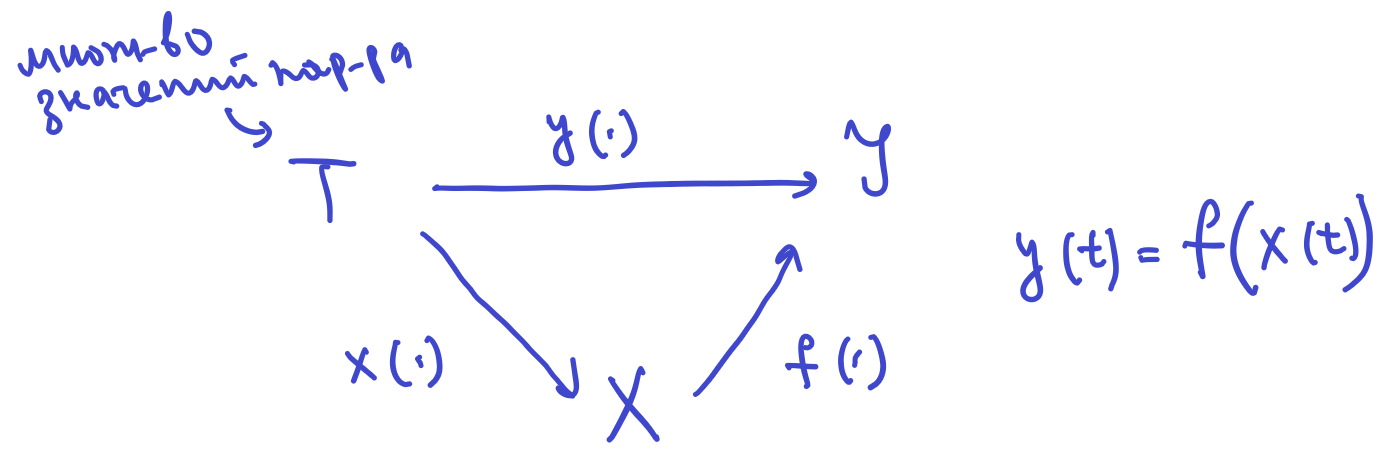
\includegraphics[width=0.8\linewidth]{images/parametric-as-function-chain}
        
        \caption{Задаваемая параметрически функция~---~это зависимость $y$ от $x$: $y \hm= f(x)$, которой в явном виде нет, но которая тем не менее ``узнаваема'' через параметр~$t$.}
        \label{fig:parametric-as-function-chain}
    \end{figure}
    
    \mbox{}\par\noindent
    \emph{Способ 1: через производные}.

    Начнём с первой производной:
    \[
      f'(x) = \frac{\diff y}{\diff x}
        = \frac{\diff y(t) / \!\diff t}{\diff x(t) / \!\diff t}
        = \frac{y'_t}{x'_t}
    \]
    \[
      f'(x) = \frac{2 t}{3 t^2} = \frac{2}{3 t}
    \]

    Вторая производная:
    \[
      f''(x) = (f')'(x) = \frac{\diff f'(x)}{\diff x}
        = \frac{\diff f'\bigl(x(t)\bigr) / \!\diff t}{\diff x(t) / \!\diff t}
    \]
    \[
      f''(x) = \frac{-2/(3t^2)}{3 t^2} = -\frac{2}{9 t^4}
    \]

    \begin{remark}
        Можно бы было получить и формулу для второй производной $f''(x)$ через производные только $x(t)$ и $y(t)$:
        \begin{equation*}
        \begin{split}
          f''(x) &= \frac{\diff f'\bigl(x(t)\bigr) / \!\diff t}{\diff x(t) / \!\diff t}\\
            &= \frac{\diff \left(\frac{\diff y(t)}{\diff x(t)}\right) / \!\diff t}{x'_t}\\
            &= \frac{1}{x'_t} \cdot \frac{\diff^2 y(t) \cdot \diff x(t) - \diff y(t) \cdot \diff^2 x(t)}{\diff x(t)^2} \Big/ \!\diff t\\
            &= \frac{1}{x'_t} \cdot \left(
              \frac{\diff\,^2 y(t)}{\diff x(t) \diff t} - \frac{\diff y(t) \diff\,^2 x(t)}{\diff x(t)^2 \diff t}
            \right)\\
            &= \frac{1}{x'_t} \cdot \left(
              \frac{\diff\,^2 y(t) / \!\diff t^2}{\diff x(t) / \!\diff t} - \frac{(\diff y(t) / \!\diff t) \cdot (\diff\,^2 x(t) / \!\diff t^2)}{\diff x(t)^2 / \!\diff t^2}
            \right)\\
            &= \frac{1}{x'_t} \cdot \left(
              \frac{y''_{tt}}{x'_t} - \frac{y'_t x''_{tt}}{x^{\prime 2}_t}
            \right)\\
            &= \frac{y''_{tt} x'_t - y'_t x''_{tt}}{x^{\prime 3}_t}
        \end{split}
        \end{equation*}
    \end{remark}

    \medskip
    
    \emph{Способ 2: через дифференциалы}.

    Пользуясь тем, что
    \[
      y(t) = f\bigl(x(t)\bigr)
    \]
    найдём первый и второй дифференциалы $y(t)$.

    Первый:
    \[
      \left\{
        \begin{aligned}
          &\diff y(t) = y'(t) \diff t\\
          &\diff y(t) = \diff f \bigl(x(t)\bigr)
            = f'(x) \diff x(t) = f'(x) x'(t) \diff t
        \end{aligned}
      \right.
    \]

    Второй:
    \[
      \diff\,^2 y(t) = \diff \bigl(\diff y(t)\bigr)
    \]
    \[
      \left\{
        \begin{aligned}
          &\diff\,^2 y(t) = \diff \bigl(y'(t) \diff t\bigr) = y''(t) \diff t^2\\
          &\diff\,^2 y(t) = \diff \bigl(f'(x) \diff x(t)\bigr)
            = f''(x) \diff x(t)^2 + f'(x) \cdot \diff\,^2 x
            = f''(x) x'^2(t) \diff t^2 + f'(x) x''(t) \diff t^2
        \end{aligned}
      \right.
    \]

    Отсюда получаем:
    \[
      \left\{
        \begin{aligned}
          &\frac{\diff\,^2 y(t)}{\diff x(t)^2}
            = \frac{y''(t) \diff t^2}{x'^2(t) \diff t^2}
            = \frac{y''(t)}{x'^2(t)}\\
          & \frac{\diff\,^2 y(t)}{\diff x(t)^2}
            = \frac{f''(x) x'^2(t) \diff t^2 + f'(x) x''(t) \diff t^2}{x'^2(t) \diff t^2}
            = f''(x) + \frac{f'(x) \cdot x''(t)}{x'^2(t)}
        \end{aligned}
      \right.
    \]

    Приравнимаем:
    \[
      \frac{y''(t)}{x'^2(t)} = f''(x) + \frac{\frac{y'(t)}{x'(t)} \cdot x''(t)}{x'^2(t)}
    \]

    Откуда получаем общее выражение для второй производной:
    \[
      \frac{\diff\,^2 f(x)}{\diff x^2} = f''(x) = \frac{x'(t) y''(t) - y'(t) x''(t)}{x'^3(t)}
    \]

    В условиях задачи:
    \[
      f'(x) = \frac{y'(t)}{x'(t)} = \frac{2}{3t}
    \]
    \[
      \frac{\diff\,^2 y(t)}{\diff x(t)^2} = \frac{y''(t)}{x'^2(t)} = \frac{2}{9 t^4}
    \]
    \[
      \frac{\diff\,^2 f(x)}{\diff x^2} = \frac{y''(t)}{x'^2(t)} - \frac{y'(t) x''(t)}{x'^3(t)}
        = \frac{2}{9 t^4} - \frac{4}{9 t^4}
        = -\frac{2}{9 t^4}
    \]

    Заметим, что в данном случае
    \[
      \frac{\diff\,^2 y(t)}{\diff x(t)^2} != \frac{\diff\,^2 f(x)}{\diff x^2}  % TODO: spacing for diff^n (should be \diff\,^n\!)
    \]
    
    Благодаря относительно аккуратным обозначениям всех участвующих в задаче функций это вроде бы и не вызывает удивления.
    Хотя если бы обозначения были такими (``попроще''):
    \[
      x = x(t),\quad y = y(t),\quad y = y(x)
    \]
    то с ними приведённое выше неравенство могло бы читаться так:
    \[
      \frac{\diff\,^2 y}{\diff x^2} != y''_{xx}
    \]
    что уже могло бы вызвать ``лёгкое'' недоумение, потому что вторая производная $y''_{xx}$ по определению вроде бы и есть $\diff\,^2 y \hm/ \diff x^2$.
  \end{solution}


  \subsection{С1, \S 15, \textnumero 22(1)}

  Найти $\diff\,^2 y$ в точке $(x_0, y_0)$ для функции $y \hm= y(x)$, заданной неявно:\footnote{
    Параметрически зададанная функция из номера~(\ref{sec:1-15-14(1)})~---~тоже есть по сути функция, заданная неявно.
    (В явном виде зависимость $y$ от $x$ не приведена.)
  }
  \[
    x^2 + 2xy + y^2 - 4x + 2y - 2 = 0,\quad (x_0, y_0) = (1, 1)
  \]
  
  \begin{solution}
    Продифференцируем обе части:
    \[
      \begin{aligned}
        &\diff \left(x^2 + 2xy + y^2 - 4x + 2y - 2\right) = 0\\
        &2x \diff x + (2 \diff x \cdot y + 2x \diff y) + 2y \diff y - 4 \diff x + 2 \diff y = 0\\
        &(2x + 2y - 4) \diff x + (2x + 2y + 2) \diff y = 0
      \end{aligned}
    \]

    В точке $(x_0, y_0) \hm= (1, 1)$:
    \[
      (2 + 2 - 4) \diff x + (2 + 2 + 2) \diff y = 0 \Rightarrow \diff y|_{(x_0, y_0)} = 0
    \]

    Продифференциуем обе части полученного ранее дифференциального соотношения:
    \[
      \begin{aligned}
        &\diff \bigl((2x + 2y - 4) \diff x + (2x + 2y + 2) \diff y\bigr) = 0\\
        &\diff (2x + 2y - 4) \diff x + \Bigl(\diff (2x + 2y + 2) \diff y + (2x + 2y + 2) \diff \bigl(\diff y\bigr)\Bigr) = 0\\
        &2 \diff x^2 + 4 \diff x \diff y + 2 \diff y^2 + (2x + 2y + 2) \diff\,^2 y = 0
      \end{aligned}
    \]

    В точке $(x_0, y_0) \hm= (1, 1)$:
    \[
      2 \diff x^2 + 0 + 0 + 6 \diff\,^2 y = 0 \Rightarrow \diff\,^2 y|_{(x_0, y_0)} = -\frac{1}{3} \diff x^2
    \]
  \end{solution}

  
  % \subsection{С1, \S 15, \textnumero 24(8)}

  \subsection{С1, \S 15, \textnumero 24(14)}\label{sec:1-15-24(14)}

  Найти $y^{(n)}(x)$ для функции:
  \[
    y = \frac{1 + x^2}{1 - x^2}
  \]
  
  \begin{solution}
    Можно бы было попробовать считать производную этот функции, смотря на неё как на произведение:
    \[
      y = \left(1 + x^2\right) \left(1 - x^2\right)^{-1}
    \]
    Но ни к чему хорошему это бы не привело: проще бы не стало~---~потому что закономерности в вычислении $n$-ой производной скобки $\left(1 - x^2\right)^{-1}$ ``не прослеживается''.

    Поэтому попробуем немного ``покрутить'' выражение, которым определяется функция.
    Так, видно, что знаменатель раскладывается на множители:
    \[
      y = \frac{1 + x^2}{(1 - x)(1 + x)}
    \]

    А дробь $\frac{1}{(1 - x)(1 + x)}$ можно разложить в сумму дробей следующим образом:
    \[
      \frac{1}{(1 - x)(1 + x)} = \frac{1}{2} \cdot \left(\frac{1}{1 - x} + \frac{1}{1 + x}\right)
    \]

    Поэтому функцию можно представить так:
    \[
      y = \frac{1}{2} \cdot \left(1 + x^2\right) \cdot \left(\frac{1}{1 - x} + \frac{1}{1 + x}\right)
    \]

    Можно ли будет теперь найти производную с помощью формулы производной произведения~\eqref{eq:diff-fg-n}?
    Да!

    Начнём с того, что найдём $n$-ые производные дробей-слагаемых.
    Первой:
    \[
      \begin{aligned}
        &\left(\frac{1}{1 - x}\right)' = (-1) \cdot \frac{1}{(1 - x)^2} \cdot (-1)\\
        &\left(\frac{1}{1 - x}\right)'' = (-1) \cdot (-2) \cdot \frac{1}{(1 - x)^3} \cdot (-1) \cdot (-1)\\
        &\ldots\\
        &\left(\frac{1}{1 - x}\right)^{(n)} = \frac{n!}{(1 - x)^{n + 1}},\quad n \geq 0
      \end{aligned}
    \]

    И второй:
    \[
      \begin{aligned}
        &\left(\frac{1}{1 + x}\right)' = (-1) \cdot \frac{1}{(1 + x)^2} \cdot 1\\
        &\left(\frac{1}{1 + x}\right)'' = (-1) \cdot (-2) \cdot \frac{1}{(1 + x)^3} \cdot 1 \cdot 1\\
        &\ldots\\
        &\left(\frac{1}{1 + x}\right)^{(n)} = \frac{(-1)^n n!}{(1 + x)^{n + 1}},\quad n \geq 0
      \end{aligned}
    \]

    Теперь можно и вернуться к производной рассматриваемой функции:
    \begin{equation*}
    \begin{split}
      y^{(n)} &= \frac{1}{2} \cdot \left(1 + x^2\right) \cdot \left(\frac{1}{1 - x} + \frac{1}{1 + x}\right)^{(n)}
        + \frac{1}{2} \cdot n \cdot \left(1 + x^2\right)' \cdot \left(\frac{1}{1 - x} + \frac{1}{1 + x}\right)^{(n - 1)}\\
        &\hphantom{MMM} + \frac{1}{2} \cdot \frac{n(n - 1)}{2} \cdot \left(1 + x^2\right)'' \cdot \left(\frac{1}{1 - x} + \frac{1}{1 + x}\right)^{(n - 2)}\\
        &= \frac{1}{2} \cdot \left(1 + x^2\right) \cdot \left(
          \frac{n!}{(1 - x)^{n + 1}} + \frac{(-1)^n n!}{(1 + x)^{n + 1}}
        \right)
        + \frac{1}{2} \cdot n \cdot 2x \cdot \left(
          \frac{(n - 1)!}{(1 - x)^{n}} + \frac{(-1)^{n - 1} (n - 1)!}{(1 + x)^{n}}
        \right)
        + \ldots
    \end{split}
    \end{equation*}

     Пожалуй, стоило бы попробовать ещё немного упростить формулу $y(x)$...

     Имеем:
     \[
       y = \frac{1}{2} \cdot \left(1 + x^2\right) \cdot \left(\frac{1}{1 - x} + \frac{1}{1 + x}\right)
     \]

     Рассмотрим дробь $\frac{1 + x^2}{1 - x}$.
     Выделим целую часть:\footnote{
       Делением в столбик.
     }
     \[
       x^2 + 1 = -x \cdot (-x + 1) + x + 1 = -x \cdot (-x + 1) - 1 \cdot (-x + 1) + 2
         \Rightarrow \frac{1 + x^2}{1 - x} = -x - 1 + \frac{2}{1 - x}
     \]

     Аналогично с дробью $\frac{1 + x^2}{1 + x}$:
     \[
       x^2 + 1 = x \cdot (x + 1) - x + 1 = x \cdot (x + 1) - 1 \cdot (x + 1) + 2
         \Rightarrow \frac{1 + x^2}{1 + x} = x - 1 + \frac{2}{1 + x}
     \]

     Поэтому функцию можно представить в таком виде:\footnote{
       Пожалуй, выделять целую часть проще бы было в самом начале, до разложения дроби в сумму дробей...
     }
     \[
       y = \frac{1}{2} \cdot \left(-x - 1 + \frac{2}{1 - x} + x - 1 + \frac{2}{1 + x}\right)
         = -1 + \frac{1}{1 - x} + \frac{1}{1 + x}
     \]

     Вот теперь уже остаётся только взять производную:
     \[
       y^{(n)} = \frac{n!}{(1 - x)^{n + 1}} + \frac{(-1)^n n!}{(1 + x)^{n + 1}},\quad n \geq 1
     \]
  \end{solution}

  
  \subsection{С1, \S 15, \textnumero 25(7)}

  Найти $y^{(n)}(x)$ для функции:
  \[
    y = x \ln{(x^2 - 3x + 2)}
  \]
  
  \begin{solution}
    Как и в задаче~\ref{sec:1-15-24(14)}, сразу напрашивается способ попробовать считать производную как производную произведения~\eqref{eq:diff-fg-n}.
    Можно попробовать, но, как и в задаче~\ref{sec:1-15-24(14)}, придётся убедиться в том, что такой способ ни к чему хорошему не приведёт...

    Что ещё можно сделать?
    Можно попробовать найти корни многочлена под логарифмом, разложить его на множители, тогда логарифм разложится в сумму логарифмов, вместо одного сложного станет два логарифма попроще, и, возможно, производную взять уже получится.
    Пойдём по этому плану.

    Разложение на множители многочлена:
    \[
      x^2 - 3x + 2 = (x - 1) (x - 2)
    \]

    Тогда формулу $y(x)$ можно переписать так:\footnote{
      Про модули можно бы было и ``забыть''~---~на последующее вычисление производной это бы не повлияло.
      Но правильно, конечно, в данном случае раскрывать логарифм с модулями.
    }
    \[
      y = x \ln{(x - 1)(x - 2)}
        = x \bigl(\ln{|x - 1|} + \ln{|x - 2|}\bigr),\quad (x - 1)(x - 2) > 0
    \]

    Теперь уже можно воспользоваться формулой для производной произведения.
    Потому что $n$-ая производная $\ln{(x - 1)}$ (и $\ln{(x - 2)}$) уже считается:
    \[
      \begin{aligned}
        &\ln'{(x - 1)} = \frac{1}{x - 1}\\
        &\ln''{(x - 1)} = \left(\frac{1}{x - 1}\right)' = (-1) \cdot \frac{1}{(x - 1)^2} \cdot 1\\
        &\ln'''{(x - 1)} = (-1) \cdot (-2) \cdot \frac{1}{(x - 1)^3} \cdot 1 \cdot 1\\
        &\ldots\\
        &\ln^{(n)}{(x - 1)} = (-1)^{n - 1} (n - 1)! \frac{1}{(x - 1)^n}
      \end{aligned}
    \]

    В результате, $n$-ая производная функции ($n \hm\geq 1$):
    % TODO: colorize
    \begin{equation*}
    \begin{split}
      y^{(n)} &= x \left(\ln^{(n)}{(x - 1)} + \ln^{(n)}{(x - 2)}\right)
          + n \cdot x' \left(\ln^{(n - 1)}{(x - 1)} + \ln^{(n - 1)}{(x - 2)}\right)\\
        &= x \left(
            (-1)^{n - 1} (n - 1)! \textcolor{pink}{\frac{1}{(x - 1)^n}} + (-1)^{n - 1} (n - 1)! \textcolor{blue}{\frac{1}{(x - 2)^n}}
          \right)\\
        &\hphantom{MMM} + n \left(
            (-1)^{n - 2} (n - 2)! \textcolor{pink}{\frac{1}{(x - 1)^{n - 1}}} + (-1)^{n - 2} (n - 2)! \textcolor{blue}{\frac{1}{(x - 2)^{n - 1}}}
          \right)\\
        &= (-1)^{n - 2} (n - 2)! \textcolor{pink}{\frac{1}{(x - 1)^{n}}} \cdot \bigl((x \cdot (-1) \cdot (n - 1) + n(x - 1)\bigr)\\
        &\hphantom{MMM} + (-1)^{n - 2} (n - 2)! \textcolor{blue}{\frac{1}{(x - 2)^{n}}} \cdot \bigl((x \cdot (-1) \cdot (n - 1) + n(x - 2)\bigr)\\
        &= (-1)^{n - 2} (n - 2)! \left(
          \frac{1}{(x - 1)^{n}} \cdot (x - n) + \frac{1}{(x - 2)^{n}} \cdot (x - 2n)
          \right)
    \end{split}
    \end{equation*}
  \end{solution}


  \section{Теоремы о среднем}

  % [X] Формулировки
  % [X] Картинки
  % [X] Пояснение Ролля и Лагранжа
  % [X] + про типы разрыва производной

  Приведём эти теоремы.

  \begin{theorem}[Ролля о среднем]\label{theo:roll}
    Пусть на отрезке $[a, b]$ определена функция~$f$, которая:
    \begin{itemize}
      \item непрерывна на $[a, b]$
      \item дифференцируема на $(a, b)$\footnote{
        Вообще говоря, также допускаются случаи, когда функция имеет в некоторых точках интервала и определённого знака \emph{бесконечную} производную~---~то есть когда её график проходит через точку ``вертикально''.
        (См. теорсправку в соответствующем параграфе (\S 16) соответствующего сборника задач (C1).)
      }
      \item принимает одинаковые значения на концах: $f(a) = f(b)$
    \end{itemize}

    Тогда найдётся точка $\xi \hm\in (a, b)$, такая что $f'(\xi) \hm= 0$~(\ref{fig:roll}).
  \end{theorem}

  \begin{figure}
      \centering
      
      \includegraphics[width=0.8\linewidth]{images/roll}
      
      \caption{Функция, удовлетворяющая условиям теоремы Ролля, и горизонтальная касательная к её графику в одной из точек.}
      \label{fig:roll}
  \end{figure}

  Почему ``работает'' теорема Ролля?\footnote{
    Не строгое доказательство.
  }
  Допустим, в точке $a$ отрезка односторонняя производная больше нуля: $f'_+(a) \hm> 0$.
  Это значит, что функция возрастает (в некоторой (полу)окрестности около $a$ будет принимать значения, большие, чем $f(a)$).
  Но она не может возрастать на всём отрезке~---~иначе она не вернётся в то же $f(b)$ значение, откуда начала ($f(b) \hm= f(a)$).
  Поэтому производная должна будет рано или поздно стать отрицательной~---~пройдя в некоторой точке через ноль?..
  Да, потому что кажется, что если допустить, что производная была сначала больше нуля, а потом сразу меньше (минуя сам ноль), то в некоторой точке будет ``излом''~(\ref{fig:corner-point})~---~то есть производной не будет, что не согласуется с условием дифференцируемости функции на всём интервале $(a, b)$.

  \begin{figure}[ht]
      \centering
      
      \includegraphics[width=0.5\linewidth]{images/corner-point}
      
      \caption{Излом графика функции~$f$ в точке~$x_0$~---~производная $f'$ в~$x_0$ не определена.}
      \label{fig:corner-point}
  \end{figure}

  Аналогичные рассуждения будут в случае, если $f'_+(a) \hm< 0$ (раз сначала убывает, то должна будет когда-нибудь и возрастать).
  Если же $f'_+(a) \hm= 0$, то либо возрастание/убывание начнётся позже, либо ещё становится возможным случай, когда просто $f'(x) \hm= 0$ на всём интервале~$(a, b)$.

  Следующая теорема является ``расширением'' теоремы Ролля.

  \begin{theorem}[Лагранжа о среднем]\label{theo:largange}
    Пусть на отрезке $[a, b]$ определена функция~$f$, которая:
    \begin{itemize}
      \item непрерывна на $[a, b]$
      \item дифференцируема на $(a, b)$
    \end{itemize}

    Тогда найдётся точка $\xi \hm\in (a, b)$, такая что:
    \[
      f'(\xi) = \frac{f(b) - f(a)}{b - a}
    \]
    то есть касательная в которой наклонена под таким же углом, как прямая, проходящая через крайние точки графика функции~$f$ на отрезке~$[a, b]$~(\ref{fig:largange}).

    Или, немного другая формулировка того же самого утверждения (с немного другим акцентом):
    \[
      f(b) = f(a) + f'(\xi) \cdot (b - a)
    \]
  \end{theorem}

  \begin{figure}
      \centering
      
      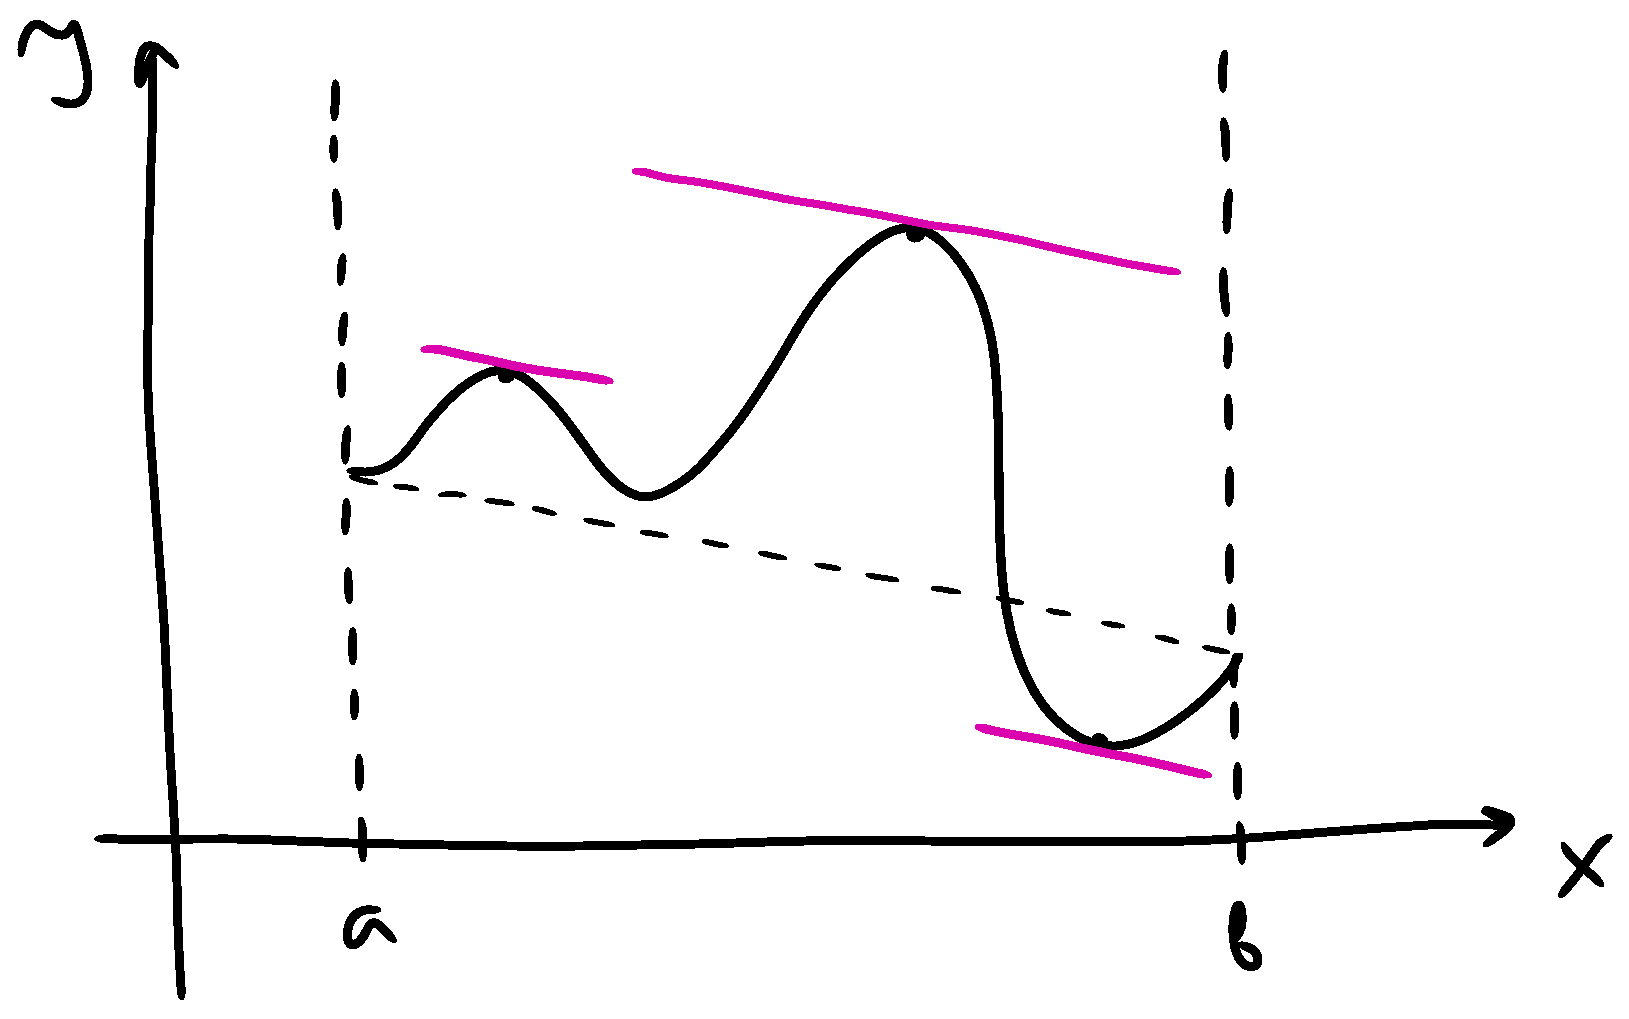
\includegraphics[width=0.8\linewidth]{images/largange}
      
      \caption{Функция, удовлетворяющая условиям теоремы Лагранжа, и касательная к её графику в одной из точек, параллельная секущей $\Bigl(\bigl(a, f(a)\bigr), \bigl(b, f(b)\bigr)\Bigr)$.}
      \label{fig:largange}
  \end{figure}

  Почему ``работает'' теорема Лагранжа?\footnote{
    Аналогично.
  }
  Ровно потому же, почему и теорема Ролля.\footnote{
    В связи между теоремами ещё можно убедиться при таком взгляде на суть утверждений: теорема Ролля говорит о том, что график функции можно заключить в ``трубку'' со стенками, параллельными оси $X$ (параллельными ``оси'' трубки~---~прямой, проходящей через точки $(a, f(a))$ и $(b, f(b))$); теорема же Лагранжа~---~утверждает то же самое, что график функции можно заключить в ``трубку'', только теперь допускаются случаи, когда ``трубка'' расположена под наклоном (ось трубки есть прямая, проходящая через точки те же точки $(a, f(a))$ и $(b, f(b))$, только теперь $f(a)$ и $f(b)$ не обязательно совпадают, в отличие от теоремы Ролля).
    (\href{https://math.stackexchange.com/questions/459406/proof-of-the-mean-value-theorem\#comment988873_459406}{Источник наблюдения}.)
  }

  Введём короткое обозначение для тангенса угла наклона секущей, проведённой через концы графика функции~$f$ на отрезке~$[a, b]$:
  \[
    c^* \equiv \frac{f(b) - f(a)}{b - a}
  \]

  Допустим, в точке $a$ отрезка односторонняя производная больше тангенса угла наклона секущей: $f'_+(a) \hm> c^*$.
  Это значит, что функция возрастает \emph{сильнее}, чем нужно для того, чтобы из точки $(a, f(a))$ попасть в точку $(b, f(b))$: если она продолжит возрастание с такой же или ещё большей скоростью, или даже если производная после точки $a$ будет всегда хотя бы не меньше $c^*$, то функция точно пройдёт ``выше'' $f(b)$ в точке~$b$.
  Поэтому производная должна будет рано или поздно стать меньше $c^*$~---~пройдя в некоторой точке через саму~$c^*$?..
  Да, иначе опять может быть ``излом''.  % TODO: pic + ref

  \begin{remark}
    Пусть функция~$f$ дифференцируема на интервале~$(a, b)$.
    Какие могут быть (и могут ли быть вообще) точки разрыва у производной $f'$?
    (Ведь не факт, что она тоже непрерывна?)

    Точки устранимого разрыва у производной быть не может: если в некоторой точке~$x_0$ имеем равенство односторонних пределов производной
    \[
      \lim_{x \to x_0 - 0} f'(x) = \lim_{x \to x_0 + 0} f'(x)
    \]
    то и сама производная~$f'(x_0)$ не может быть равна ничему другому, кроме как этому пределу.
    (Потому что в этом случае будут существовать односторонние производные, каждая из которых будет равна соответствующему пределу производной.)\footnote{
      Покажем, что если у функции~$f$ существует односторонний предел производной в точке~$x_0$, например:
      \[
        \exists \lim_{x \to x_0 + 0} f'(x)
      \]
      то в этом случае будет существовать и соответствующая односторонняя производная~$f'_+(x_0)$ в этой точке, причём:
      \[
        f'_+(x_0) = \lim_{x \to x_0 + 0} f'(x)
      \]

      Заметим, что вопрос по сути сводится к тому, можно ли ``переставить'' пределы:
      \begin{equation*}
      \begin{split}
        \lim_{x \to x_0 + 0} f'(x) &= \lim_{x \to x_0 + 0} \lim_{z \to x} \frac{f(z) - f(x)}{z - x}\\
          &\overset{\?}{=} \lim_{z \to x} \lim_{x \to x_0 + 0} \frac{f(z) - f(x)}{z - x}
          \overset{\?}{=} \lim_{z \to x_0 + 0} \frac{f(z) - f(x_0)}{z - x_0}
          = f'_+(x_0)
      \end{split}
      \end{equation*}

      Пусть (для краткости):
      \[
        \lim_{x \to x_0 + 0} f'(x) \equiv A
      \]

      \textbf{Что имеем}:
      \[
        \forall \eps > 0\ \exists \delta > 0\colon \forall x \in U_{+\delta}(x_0) \to f'(x) \in U_{\eps}(A)
      \]
      где за $U_{+\delta}(x_0)$ обозначена правая половинка $\delta$-окрестности~$x_0$.
      При этом производная $f'(x)$ есть:
      \[
        f'(x) = \lim_{z \to x} \frac{f(z) - f(x)}{z - x} \equiv A_x
      \]
      и раз эта производная существует, то можно также записать:
      \[
        \forall \widetilde \eps\ \exists \widetilde \delta\colon \forall z \in U_{\widetilde \delta}(x) \to \frac{f(z) - f(x)}{z - x} \in U_{\widetilde \eps}(A_x)
      \]

      Итак, собирая всё вместе:
      \[
        \left\{
          \begin{aligned}
            &\left|\frac{f(z) - f(x)}{z - x} - A_x\right| < \widetilde \eps, & &z \in U_{\widetilde \delta}(x)\\
            &|A_x - A| < \eps, & &x \in U_{+\delta}(x_0)
          \end{aligned}
        \right.
      \]

      Откуда получаем (просто ``замечаем''~---~пока не понятно, пригодится ли это вообще):
      \[
        \left|\frac{f(z) - f(x)}{z - x} - A\right| < \eps + \widetilde\eps,\quad x \in U_{+\delta}(x_0),\ z \in U_{\widetilde \delta}(x)
      \]
      (по сути это означает, что модуль разности в левой части можно сделать сколь угодно маленьким~---~так как $\eps$ и $\widetilde\eps$ произвольные больше нуля).

      \textbf{Что хотим}:
      \[
        \lim_{z \to x_0 + 0} \frac{f(z) - f(x_0)}{z - x_0} \overset{\?}{=} A
      \]

      Это равносильно:
      \[
        \forall \widehat\eps > 0\ \exists \widehat\delta > 0\colon \forall z \in U_{+{\widehat\delta}}(x_0) \to \frac{f(z) - f(x_0)}{z - x_0} \in U_{\widehat\eps}(A)
      \]
      % \bar\eps fails (100 errors "number expected -- treated as zero")

      Теперь ``соединяем'': что есть~---~с тем, что хотим получить:
      \begin{equation}\label{eq:in-footnote}   
        \left|\frac{f(z) - f(x_0)}{z - x_0} - A\right|
          \leq \left|\frac{f(z) - f(x_0)}{z - x_0} - \frac{f(z) - f(x)}{z - x}\right| + \left|\frac{f(z) - f(x)}{z - x} - A\right|
      \end{equation}
      (где $x$ есть некоторая точка из некоторой окрестности $U_{+\delta}(x_0)$, а $z$ при этом находится рядом с ней: $z \hm\in U_{\widetilde\delta}(x)$~---~итого, при достаточно малой $\widetilde\delta$ точка~$z$ также лежит правее~$x_0$).

      Второй модуль разности справа не больше $\eps \hm+ \widetilde\eps$ (уже показали выше).
      А что с первым модулем разности?
      Его тоже можно сделать сколь угодно маленьким!
      Потому что $x \hm\approx x_0$ (можно считать, что $x$ расположен к $x_0$ так близко, как хотим~---~с любой желаемой наперёд заданной ``точностью''), а ввиду непрерывности функции~$f$ также имеем $f(x) \hm\approx f(x_0)$ (причём выбирая $x$ всё ближе к $x_0$ получаем одновременно и $f(x)$ всё ближе к $f(x_0)$).
      А значит, $z \hm- x \hm\approx z \hm- x_0$, и $f(z) \hm- f(x) \hm\approx f(z) \hm- f(x_0)$.
      А потому и
      \[
        \frac{f(z) - f(x_0)}{z - x_0} \approx \frac{f(z) - f(x)}{z - x}
      \]
      то есть первый модуль разности в~\eqref{eq:in-footnote} выбором окрестности $\delta$ также можно сделать сколь угодно маленьким.

      Итого, в некоторой окрестности~$x_0$ (зависящей от $\delta$, $\widetilde\delta$ и от близости между $x$ и $x_0$, необходимой для достаточной малости ``первого модуля разности'')
      \[
        \left|\frac{f(z) - f(x_0)}{z - x_0} - A\right| < \widehat\eps
      \]
      для произвольного $\widehat\eps \hm> 0$.
    }

    Точки разрыва первого рода у производной также быть не может: если в некоторой точке~$x_0$ существуют пределы производной слева $\lim_{x \to x_0 - 0} f'(x)$ и справа $\lim_{x \to x_0 + 0} f'(x)$, но они не равны, то производной в точке $x_0$ не существует.
    (Что противоречит тому, что по условию функция~$f$ должна быть дифференцируема на всём $(a, b)$.)

    Остаётся разрыв второго рода: когда в некоторой точке $x_0$ не существует (конечного) предела производной слева или справа.
    Такие разрывы у производной могут быть.
  \end{remark}
  
  % For the history
% \iffalse  % 1756(ok) - 1862(fail)

  \begin{example}  % https://www.rsdn.org/forum/etude/1070903.all
    Рассмотрим функцию~(\ref{fig:func-with-diff-break}):
    \begin{equation}\label{eq:func-with-diff-break}
      f(x) = \left\{
        \begin{aligned}
          &x^2 \sin{\left(\frac{1}{x}\right)} & &x \not= 0\\
          &0 & &x = 0
        \end{aligned}
      \right.
    \end{equation}

    \begin{figure}[ht]
      \centering
    
      \begin{subfigure}[b]{0.8\textwidth}
        \centering
    
        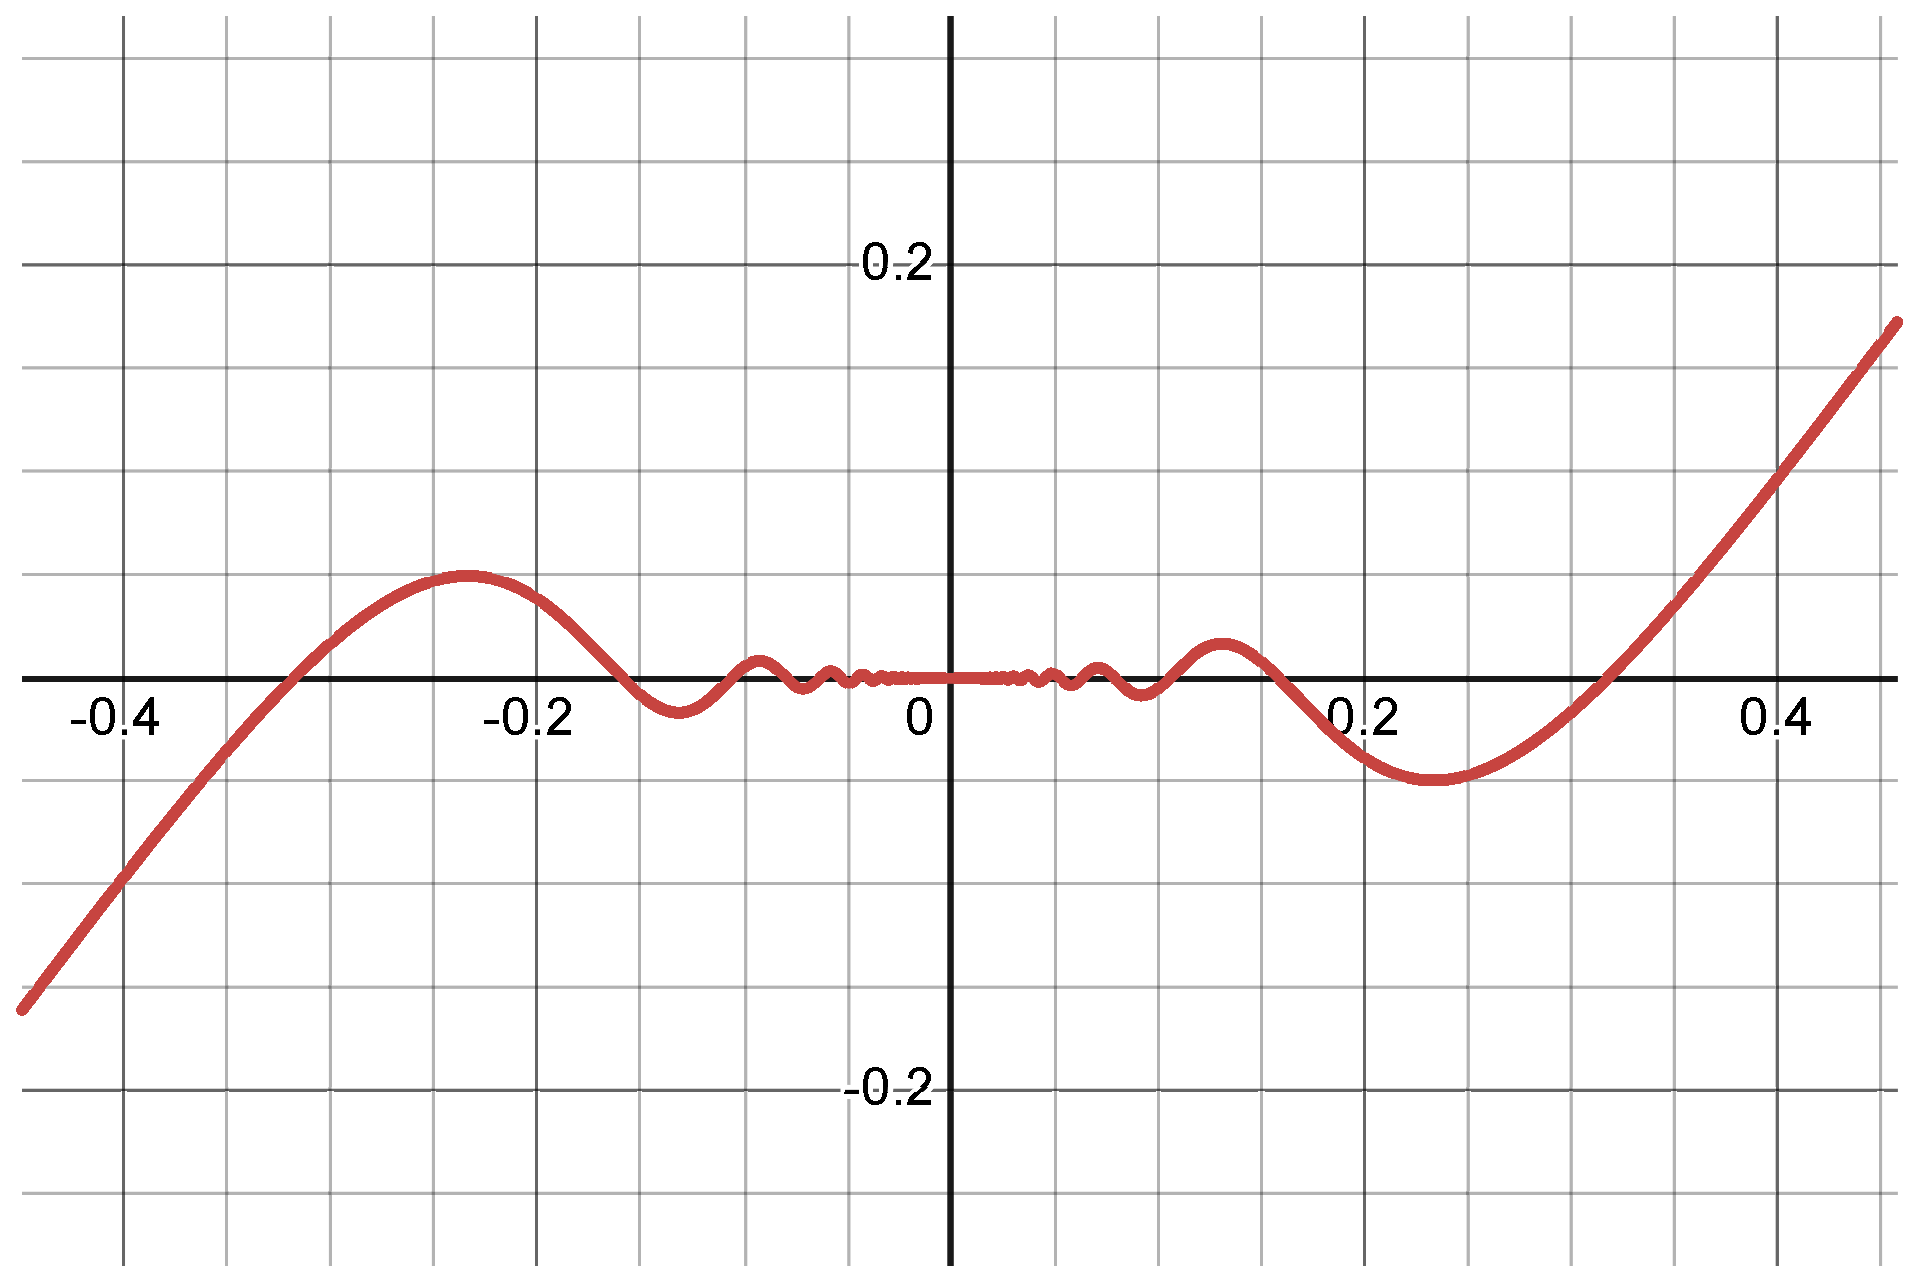
\includegraphics[width=\columnwidth]{images/x2sinx-1}
    
        \caption{``Взгляд сверху''.}
      \end{subfigure}
      % \hfill
      \begin{subfigure}[b]{0.8\textwidth}
        \centering
        
        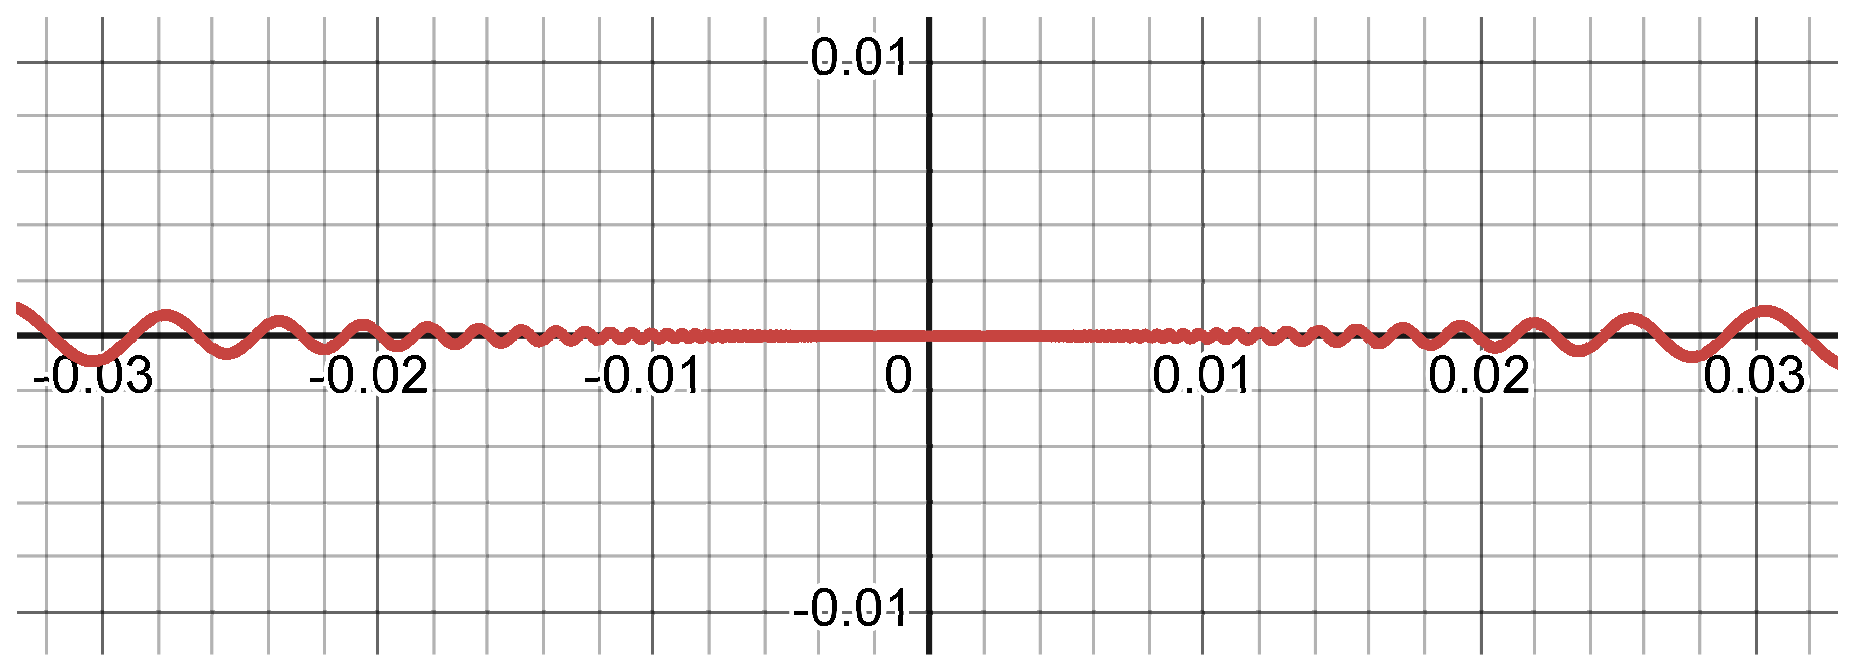
\includegraphics[width=\columnwidth]{images/x2sinx-1_zoom}
  
        \caption{``Зум'' в область около нуля.}
      \end{subfigure}
    
      \caption{График функции~\eqref{eq:func-with-diff-break}.}
      \label{fig:func-with-diff-break}
    \end{figure}


    Её производная:
    \[
      f'(x) = 2x \sin{\left(\frac{1}{x}\right)} - \cos{\left(\frac{1}{x}\right)},\quad x \not= 0
    \]

    В нуле:
    \[
      f'(0) = \lim_{x \to 0} \frac{x^2 \sin{\left(\frac{1}{x}\right)} - 0}{x} = 0
    \]

    Очевидно, что
    \[
      \not\exists \lim_{x \to 0} f'(x)
    \]
    то есть в нуле производная~$f'$ терпит разрыв второго рода.
  \end{example}

  Излома у функции быть не может, потому что это соответствует разрыву первого рода производной, что невозможно.
  Но у производной может быть разрыв второго рода~---~может быть, производная всё-таки может ``проскочить'' $c^*$?..
  
  Итак, начнём сначала.\footnote{
    Более строгое доказательство.
  }
  На отрезке $[a, b]$ найдутся две точки $l$ и $r$, такие что $f'(l) \hm< c^*$ и $f'(r) \hm> c^*$ (или наоборот)~---~в противном случае $f'(x) \hm= c^*$ на всём отрезке.
  Рассмотрим отрезок $[l, r] \equiv [l_1, r_1]$.
  В точке~--~середине отрезка $m_1 \equiv \frac{l_1 + r_1}{2}$ возможны случаи: $f'(m_1) \hm> c^*$, $f'(m_1) \hm= c^*$ и $f'(m_1) \hm< c^*$.
  Во втором случае поиск закончен.
  В первом~---~переходим к новому отрезку $[l_2, r_2] \hm= [l_1, m_1]$, в третьем~---~к отрезку~$[m_1, r_1]$.
  И так далее.
  В общем случае получаем стягивающуюся последовательность вложенных отрезков $\bigl\{[l_n, r_n]\bigr\}$.
  Стягивающуюся в некоторую точку $x^*$.
  При этом имеем:
  \[
    \left\{
      \begin{aligned}
        &f'(l_n) < c^*\\
        &f'(r_n) > c^*
      \end{aligned}
    \right.\quad n = 1, 2, \ldots
  \]

  Что можно сказать про $f'(x^*)$?\footnote{
    Из симметрии всей ситуации кажется, что не остаётся никаких вариантов, кроме $f'(x^*) \hm= c^*$ ...или варианта, когда $f'(x^*)$ может быть как больше, так и меньше $c^*$ (когда оба неравенства возможны и однозначно определить ``правильное'' в общем случае нельзя).
  }
  Если в точке $x^*$ производная непрерывна, то сразу получаем $f'(x^*) = c^*$.\footnote{
    Как в теореме о промежуточном значении непрерывной на отрезке функции.
  }
  Если в точке $x^*$ производная разрывна, то это точно разрыв второго рода...
  % Допустим, $f'(x^*) \hm< c^*$.
  % Что это означает?
  % Что в некоторой полуокрестности слева от $x^*$ верно, что
  % \[
  %   \frac{f(x^*) - f(x)}{x^* - x} < c^*
  %     \quad\Leftrightarrow\quad f(x) > f(x^*) - c^* \cdot (x^* - x)
  % \]
  % а в некоторой полуокрестности справа верно, что
  % \[
  %   \frac{f(x) - f(x^*)}{x - x^*} < c^*
  %     \quad\Leftrightarrow\quad f(x) < f(x^*) + c^* \cdot (x - x^*)
  % \]
  Может ли $f'(x^*) \hm{\not=} c^*$ (а быть больше либо меньше $c^*)$? не получится ли в этом случае какого-нибудь противоречия?..
  Размышления приводят к заключению, что в возможном отличии $f'(x^*)$ от $c^*$ ничего плохого нет.
  Более того, можно просто предложить функцию, у которой в некоторой точке у производной будет разрыв второго рода, а сама производная в этой точке может принимать любое наперёд заданное значение~(\ref{fig:any-diff-at-break}).
  
% \iffalse % 1956

  \begin{figure}[ht]
      \centering
      
      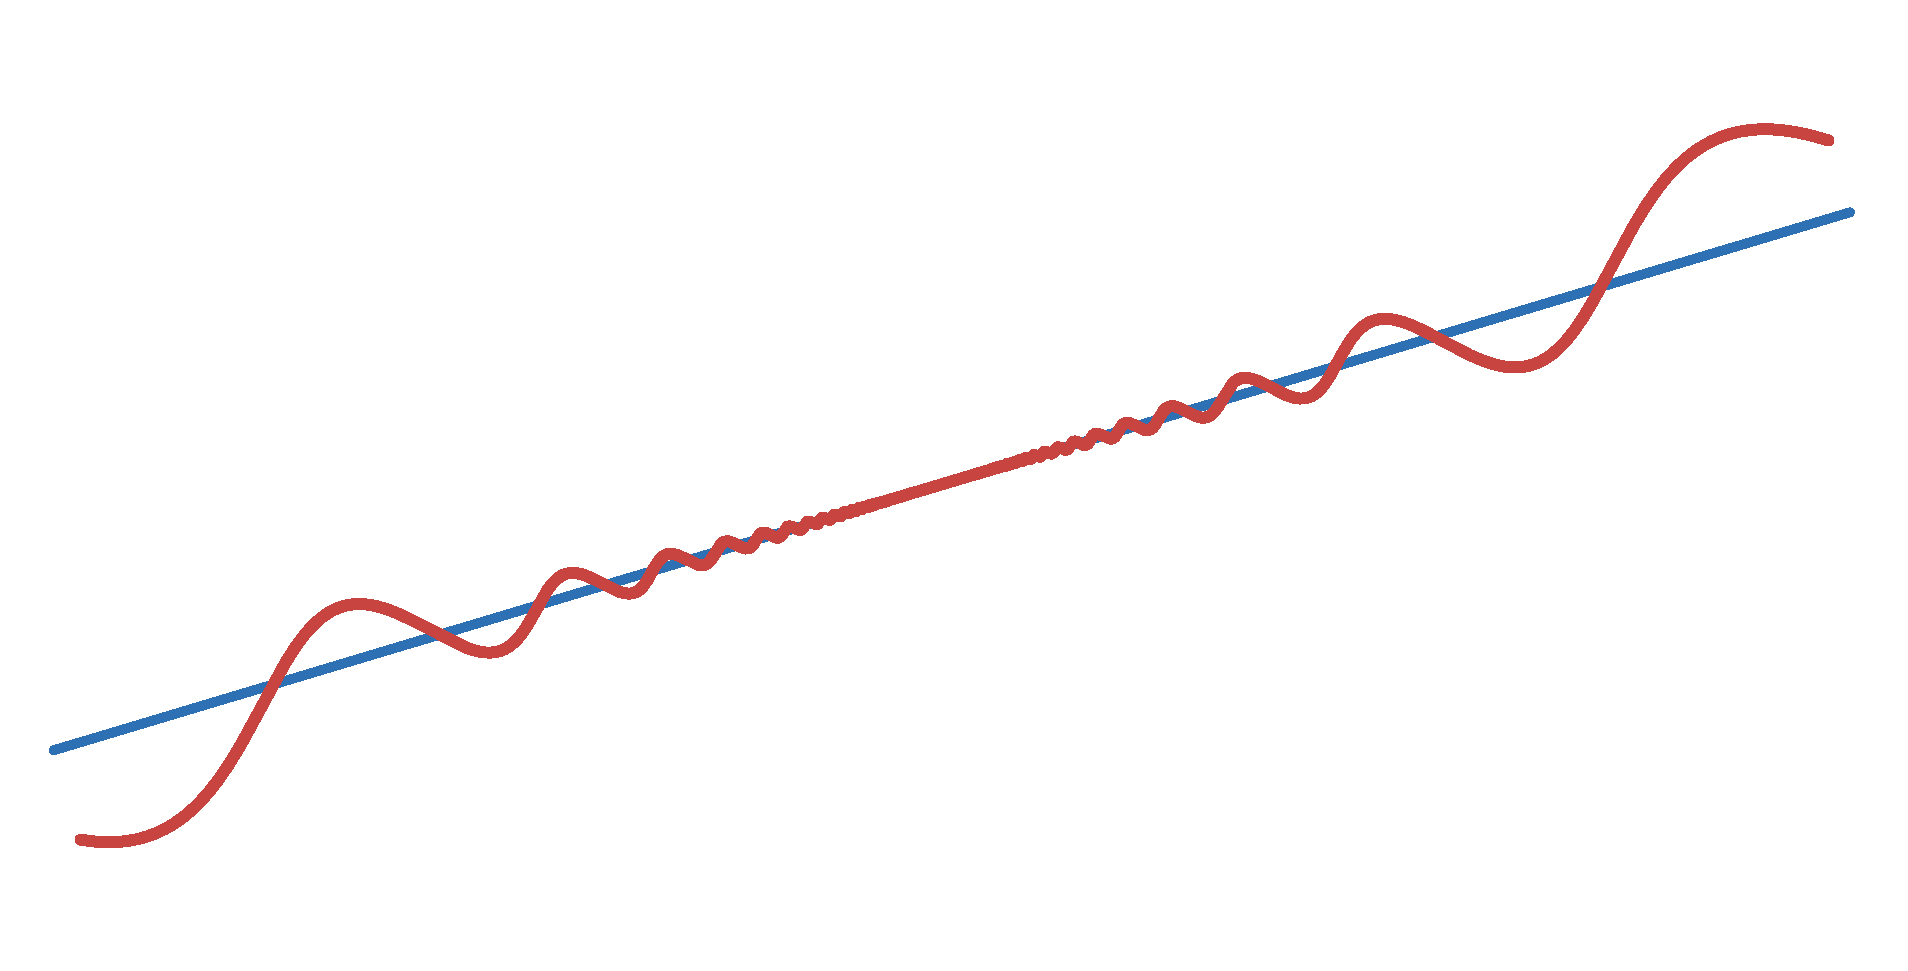
\includegraphics[width=0.8\linewidth]{images/func-with-any-diff-at-break3}
      
      \caption{``Эскиз'' ситуации, когда у функции (красный график) в некоторой точке есть разрыв производной, но значение производной в этой точке при этом (синяя прямая) какое-нибудь любое заранее заданное ненулевое (очевидно, можно нарисовать синюю прямую под любым углом, а потом как-нибудь аккуратно организовать ``бесконечный волнообразный спад'' в точку около этой прямой.}
      \label{fig:any-diff-at-break}
  \end{figure}

  Итак, в точке $x^*$ может быть разрыв производной, и поиск $c^*$ завершается неудачно...
  Что можно сделать в этом случае?
  Предлагается такой ``обходной путь''.
  Пусть $x^* \hm\equiv x^*_1$.
  Если $f'(x^*_1) \hm> c^*$, то положим $[\widetilde l_1, \widetilde r_1] \hm\equiv [l_1, x^*_1]$; если же $f'(x^*_1) \hm< c^*$, то положим $[\widetilde l_1, \widetilde r_1] \hm\equiv [x^*, r_1]$.  % [\tilde l_1, \tilde r_1] fails (100 errors)
  И далее будем стягивать по описанной ранее процедуре делением пополам отрезок $[\widetilde l_1, \widetilde r_1]$!
  Он стянется в некоторую точку~$x^*_2$, в которой опять либо производная будет непрерывна и равна $c^*$ (и на этом конец), либо будет разрывна и равна $c^*$ (тоже конец), либо... будет разрывна и не равна $c^*$.
  В случае очередного ``неудачного стягивания''~---~снова переходим к новому начальному отрезку, стягиваем его, получаем точку, и так далее.
  В общем случае ``неудачных'' точек стягивания может получиться бесконечно много (может получиться последовательность таких точек $\left\{x^*_n\right\}$): в каждой из которых у производной $f'$ наблюдается разрыв второго рода, но значение производной не равно~$c^*$.
  По теореме Больцано~--~Вейерштрасса, из такой последовательности (ограниченной) можно будет выделить сходящуюся подпоследовательность~---~подпоследовательность~$\left\{x^*_{n_k}\right\}$ из точек разрыва производной~$f'$ второго рода, сходящуюся к некоторой точке $z^* \hm\in (a, b)$.
  Что можно сказать про эту точку~$z^*$?\footnote{
    Будет ли в ней наконец выполняться $f'(z^*) = c^*$? ':D  % TODO tikz something? https://tex.stackexchange.com/a/227226/135045
  }
  Может ли она, например, также быть точкой разрыва второго рода производной?
  Кажется, что да~(\ref{fig:func-with-accumulation-break-diff-point}).
  Более того, кажется, что $f'(z^*)$ в общем случае может быть любой...

  \begin{figure}[ht]
      \centering
      
      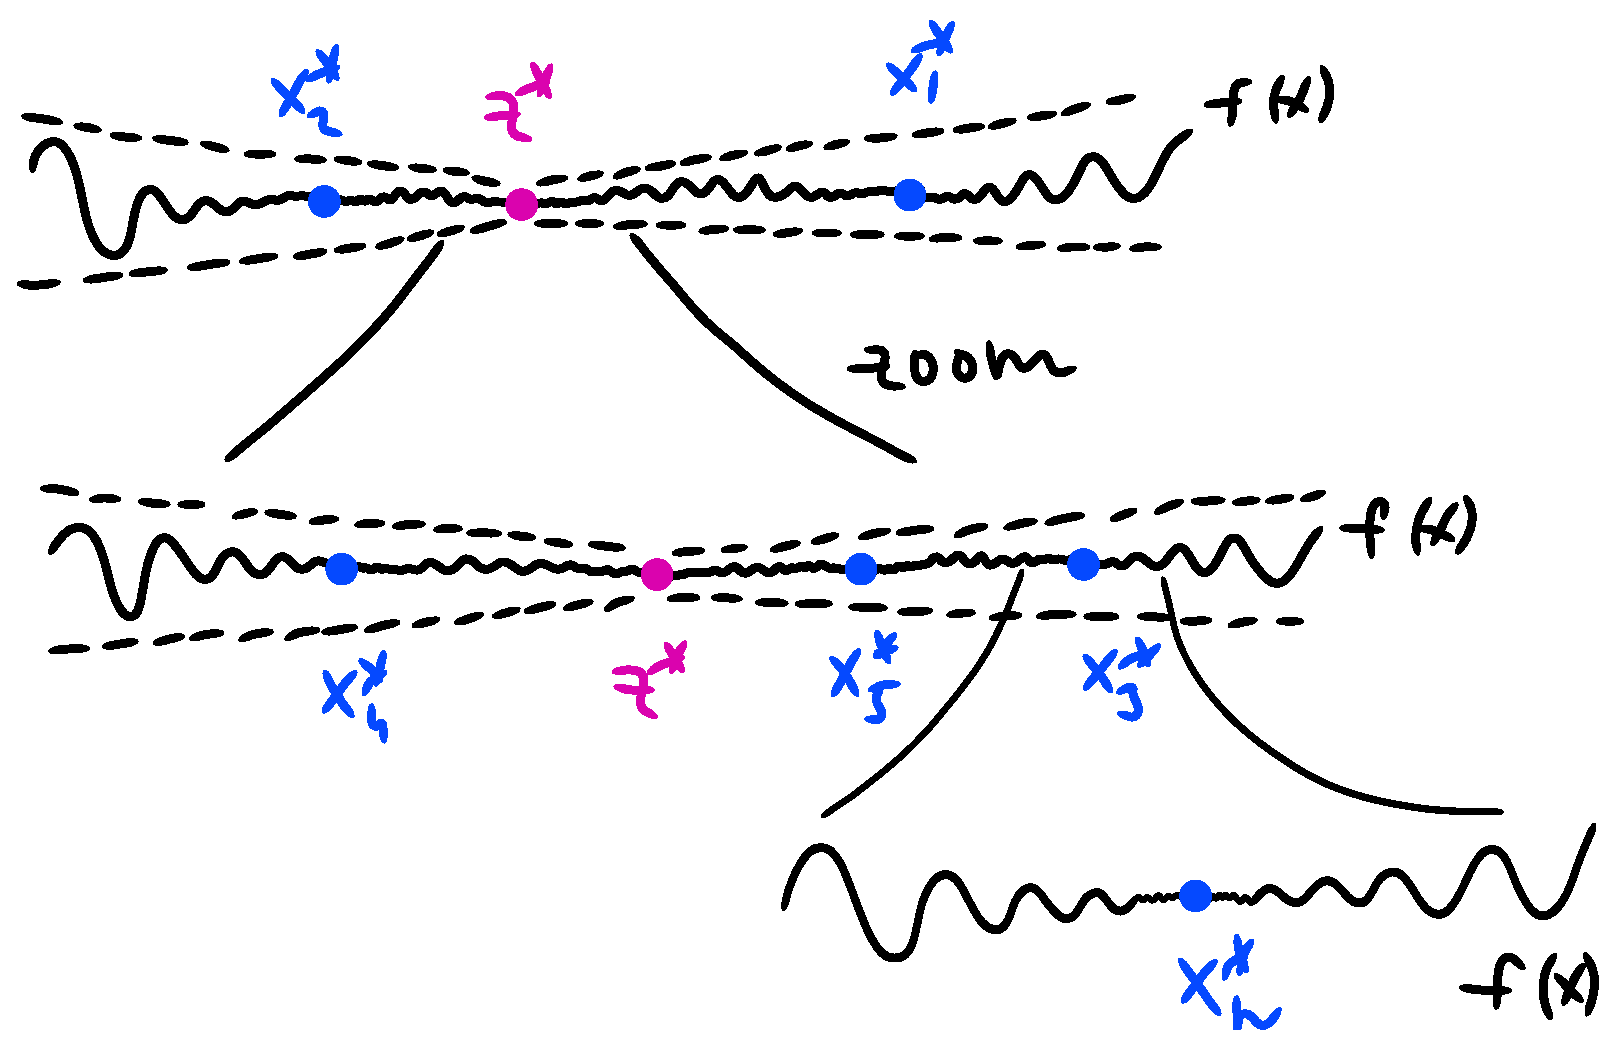
\includegraphics[width=0.8\linewidth]{func-with-accumulation-break-diff-point}
      
      \caption{``Эскиз'' ситуации, когда у функции есть последовательность точек разрыва второго рода производной, которая сходится к точке~---~также разрыву второго рода производной.
      (Развитие примера~(\ref{fig:any-diff-at-break}).)}
      \label{fig:func-with-accumulation-break-diff-point}
  \end{figure}

  Предлагается на этом закончить текущее ``доказательство''.

  Однако отметим, что если к условиям из теоремы Лагражна добавить \emph{ещё одно}, состоящее в том, что у функции~$f$ может быть лишь \emph{конечное} число точек разрыва производной на интервале~$(a, b)$,\footnote{
    Строгое ли это условие?
    Или, другими словами~---~много ли читатель знает функций, у которых производная имела бы бесконечное число точек разрыва на каком-нибудь интервале?
  } то представленное выше рассуждение из ``доказательства'' в самом деле становится доказательством.
  (\emph{Последовательности} $\left\{x^*_n\right\}$ не получится~---~на каком-то шаге очередная точка~$x^*_k$ окажется точкой непрерывности производной и в ней будет достигнуто $f'(x^*_k) \hm= c^*$.)
  Более того, это уже будет не просто доказательство \emph{существования} нужной точки (где касательная наклонена под определённым углом), но ещё и алгоритм \emph{поиска} такой точки.

  % https://math.stackexchange.com/questions/459406/proof-of-the-mean-value-theorem

  \begin{remark}
    Для полноты картины представим более адекватный (стандартный) способ доказательства теоремы Лагранжа (и Ролля).

    Раз функция~$f$ непрерывна на $[a, b]$, то она достигает на нём своих верхней и нижней граней (конечных).
    Пусть, например, $f(x^*) \hm= \sup_{[a, b]} f$.
    Если значения на концах отрезка у функции совпадают, а сама она не константная, то $x^* \hm\in (a, b)$ (то есть точка, где достигается супремум, лежит внутри отрезка).
    Так как функция~$f$ дифференцируема на интервале $(a, b)$, то она дифференцируема и в $x^*$, причём $f'(x^*) \hm= 0$, так как
    \[
      \begin{aligned}
        &f(x) - f(x^*) \leq 0 & &\mbox{для всех точек правее } x^*\\
        &f(x^*) - f(x) \geq 0 & &\mbox{для всех точек левее } x^*\\
      \end{aligned}
      \Rightarrow
      \begin{aligned}
        &f'_+(x^*) \leq 0\\
        &f'_-(x^*) \geq 0\\
      \end{aligned}
      \Rightarrow
      f'(x^*) = 0
    \]
    Это доказывает теорему Ролля.

    Если же функция~$f$ принимает разные значения на концах, то на её основе можно определить \emph{новую} непрерывную на $[a, b]$ функцию, такую чтоб у неё уже значения на концах совпадали.
    Например, искать эту функцию можно в виде: $g(x) \hm= f(x) - \alpha \hm\cdot x$.
    Из условия $g(a) \hm= g(b)$ получается коэффициент $\alpha \hm= \frac{f(b) - f(a)}{b - a}$.
    А теорема Ролля в применении к~$g$ даёт наличие точки~$\xi$, где $g'(\xi) \hm= 0$, а потому $f'(\xi) \hm= \frac{f(b) - f(a)}{b - a}$.
  \end{remark}

  И последняя теорема о среднем.

  \begin{theorem}[Коши о среднем]\label{theo:cochi}
    Пусть на отрезке $[a, b]$ определены функции $x \hm= \phi(t)$ и $y \hm= \psi(t)$, причём:
    \begin{itemize}
      \item $\phi(t)$ и $\psi(t)$ непрерывна на $[a, b]$
      \item $\phi(t)$ и $\psi(t)$ дифференцируемы на $(a, b)$
      \item $\phi'(t) \hm{\not=} 0$\footnote{
        Отсюда же по теореме Ролля следует, что $\phi(a) \hm{\not=} \phi(b)$.
      }\textsuperscript{,}\footnote{
        Это условие можно ослабить или даже вообще опустить (если переписать формулу из теоремы в виде равенства произведений, а не в виде пропорции).
      }
    \end{itemize}

    Тогда найдётся точка $\xi \in (a, b)$, такая что\footnote{
      Касательная в ней к графику параметрически заданной кривой будет параллельна секущей, соединяющей начало и конец графика кривой на отрезке.
    }
    \[
      \frac{\psi'(\xi)}{\phi'(\xi)} = \frac{\psi(b) - \psi(a)}{\phi(b) - \phi(a)}
    \]
  \end{theorem}

  %В более общей (требующей меньше условий) записи:
  %\[
    %\psi'(\xi) \cdot \bigl(\phi(b) - \phi(a)\bigr)
      %= \phi'(\xi) \cdot \bigl(\psi(b) - \psi(a)\bigr)
  %\]



  \subsection{С1, \S 16, \textnumero 5}

  Доказать, что если функция~$f$ дифференцируема~$n$ раз на отрезке~$[a, b]$ и обращается на нём в ноль в $n \hm+ 1$ точках, то найдётся $\xi \hm\in (a, b)$, такая что $f^{(n)}(\xi) \hm= 0$.
  
  \begin{solution}
    Функция обращается на отрезке~$[a, b]$ в ноль в $n \hm+ 1$ точках~---~значит, весь отрезок нулями функции разбивается на~$n$ подотрезков, на каждом из которых функция~$f$ удовлетворяет условиям теоремы Ролля~(\ref{theo:roll}).
    Поэтому найдётся~$n$ точек, где обращается в ноль производная $f'(x)$.
    
    А это значит, что весь отрезок~$[a, b]$ нулями производной разбивается на~$n \hm- 1$ подотрезков, на каждом из которых производная функции~$f'$ удовлетворяет условиям теоремы Ролля.
    Поэтому найдётся~$n \hm- 1$ точка, где обращается в ноль производная производной, то есть $f''(x)$.
    
    А это значит, что...
    И так далее.
    Очевидно, цепочку рассуждений можно аналогичным образом продолжать.
    Получается, что:
    \[
      \begin{aligned}
        &f           & &n + 1\ \mbox{нулей}\\
        &f'          & &n\ \mbox{нулей}\\
        &f''         & &n - 1\ \mbox{нулей}\\
        &\ldots      & &{}\\
        &f^{(n - 1)} & &2\ \mbox{нуля}\\
        &f^{(n)}     & &1\ \mbox{ноль}\quad \Smiley  % https://tex.stackexchange.com/a/227226/135045
      \end{aligned}
    \]
  \end{solution}


  \subsection{С1, \S 16, \textnumero 15(3)}

  Пользуясь теоремой Лагранжа, доказать неравенство:
  \[
    e^x \geq 1 + x,\quad x \in \RR
  \]
  
  \begin{solution}
    (Графически убеждаемся, что неравенство~---~правда.)

    Что говорит теорема Лагранжа?
    Один из вариантов её ``прочитать'' такой.
    Что для ``хорошей'' функции~$f$ верно, что её значение в некоторой точке~$x$ можно представить таким образом (через ``поправку'' к значению в какой-то другой точке~$x_0$):
    \begin{equation}\label{eq:1-16-15(3)}
      f(x) = f(x_0) + f'(\xi) \cdot (x - x_0),\quad \xi\ \mbox{между } x\ \mbox{и } x_0
    \end{equation}

    Определим в качестве функции $f$:
    \[
      f(x) \equiv e^x - 1 - x
    \]

    А в качестве $x_0$ возьмём, например: $x_0 \hm= 0$.

    Тогда имеем:
    \[
      \left\{
        \begin{aligned}
          &f(x_0) = \left(e^x - 1 - x\right)|_{x = x_0} = 0\\
          &f'(x) = e^x - 1\\
        \end{aligned}
      \right.
    \]
    и, по теореме Лагранжа~\eqref{eq:1-16-15(3)}:
    \[
      e^x - 1 - x = 0 + \left(e^{\xi} - 1\right) \cdot x
    \]

    Если $x \hm> 0$, то правая часть тоже больше нуля (таким образом, $e^x \hm- 1 \hm- x \hm> 0$).
    Если $x \hm= 0$, то обе части зануляются.
    Если $x \hm< 0$, то правая часть снова становится больше нуля.
    Итого, объединяя все случаи, получаем:
    \[
      e^x - 1 - x \geq 0
        \quad\Leftrightarrow\quad e^x \geq 1 + x
    \]

    \medskip

    Можно бы было попробовать взять в качестве функции из теоремы Лагранжа какую-нибудь другую.
    Например:
    \[
      g(x) \equiv e^x
    \]
    ``Начальную точку'' $x_0$ оставим прежней ($x_0 \hm= 0$).
    Тогда можем записать:
    \[
      \begin{aligned}
        &g(x) = g(x_0) + g'(\xi) \cdot (x - x_0)\\
        &e^x = 1 + e^{\xi} \cdot x
      \end{aligned}
    \]

    Очевидно, при $x \hm> 0$ будет:
    \[
      1 + e^{\xi} \cdot x > 1 + x
    \]
    При $x \hm= 0$ будет равенство, при $x \hm< 0$ снова будет знак ``больше''.
    Поэтому в итоге снова получаем $e^x \hm\geq 1 \hm+ x$.
  \end{solution}


  \subsection{С1, \S 16, \textnumero 19}

  Доказать, что если функция~$f$ дифференцируема и неограничена на конечном интервале~$(a, b)$, то её производная также неограничена на этом интервале.
  
  \begin{solution}
    \begin{figure}
        \centering
        
        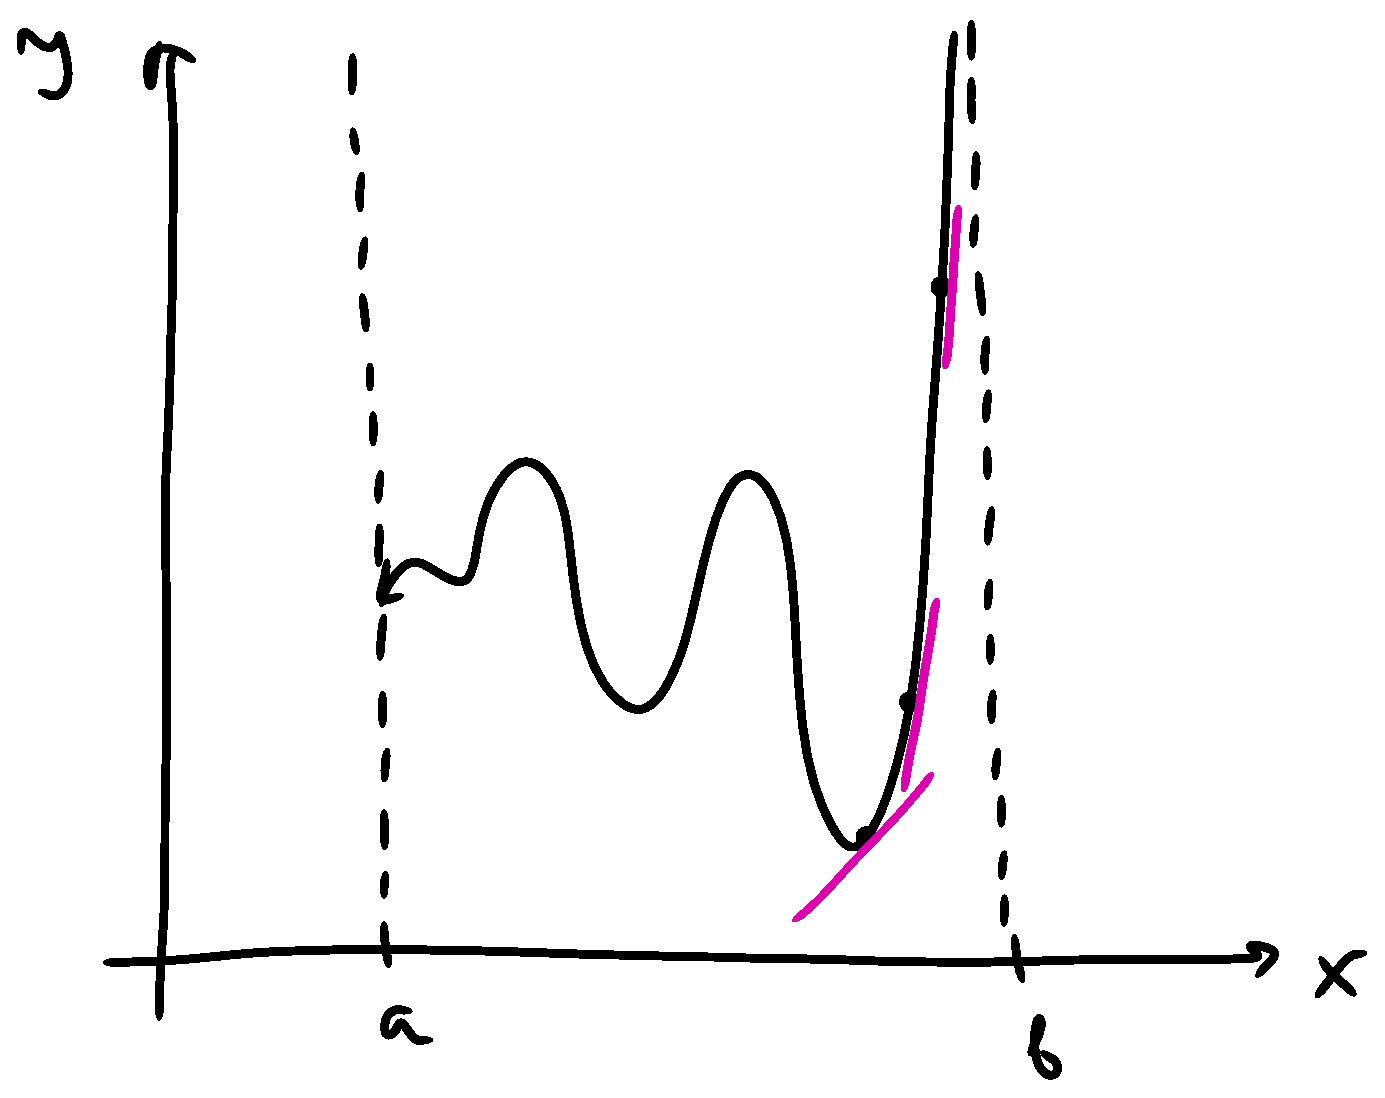
\includegraphics[width=0.8\linewidth]{images/unlimited-func}
        
        \caption{Функция, неограниченная на интервале~$(a, b)$.}
        \label{fig:unlimited-func}
    \end{figure}

    Графически утверждение кажется понятным~(\ref{fig:unlimited-func}).
    Как доказать более строго?
    При движении по графику функции в сторону, где она бесконечно возрастает, её производная становится всё ``круче''...

    Применим теорему Лагранжа.
    Пусть~$x_0$~---~некоторая точка интервала.
    Тогда для произвольной $x$ из интервала можно записать (при некоторой $\xi$ лежащей между $x_0$ и $x$):
    \[
      f(x) = f(x_0) + f'(\xi) \cdot (x - x_0)
    \]

    Так как функция $f$ неограничена на интервале, значение $f(x)$ может каким угодно большим.
    Если же допустить, что производная ограничена ($|f'(\xi)| \hm\leq C$, $\forall \xi \hm\in (a, b)$), то и вся правая часть будет ограничена:
    \[
      \bigl|f(x_0) + f'(\xi) \cdot (x - x_0)\bigr| \leq |f(x_0)| + C \cdot (b - a)
    \]
    Что означает противоречие.

    Иначе, можно бы было просто из теоремы Лагранжа выразить значение производной в точке~$\xi$:
    \[
      f'(\xi) = \frac{f(x) - f(x_0)}{x - x_0},\quad x \not= x_0
    \]
    Числитель дроби справа неограничен по величине, знаменатель ограничен, итого производная неограничена.
  \end{solution}


  \subsection{С1, \S 16, \textnumero 33}

  Выяснить, будет ли всегда существовать точка~$\xi \hm\in (a, b)$, такая что $f'(\xi) \hm= 0$, если функция~$f$ удовлетворяет всем условиям теоремы Ролля~(\ref{theo:roll}), кроме одного из следующих:
  \begin{itemize}
    \item функция~$f$ непрерывна на отрезке~$[a, b]$
    \item функция~$f$ имеет во всех точках интервала~$(a, b)$ конечную или определённого знака бесконечную производную
    \item $f(a) = f(b)$
  \end{itemize}
  
  \begin{solution}
    Вместо слов, приведём по картинке-контрпримеру на каждый из пунктов:
    первый~(\ref{fig:1-16-33-a}), второй~(\ref{fig:1-16-33-b}) и третий~(\ref{fig:1-16-33-c}).

    \begin{figure}[ht]
      \centering
    
      \begin{subfigure}[b]{0.32\textwidth}
        \centering
    
        \includegraphics[width=\columnwidth]{images/not-roll-a}
    
        \caption{Без непрерывности функции на отрезке теорема Ролля может не работать.}
        \label{fig:1-16-33-a}
      \end{subfigure}
      %
      \hfill
      %
      \begin{subfigure}[b]{0.32\textwidth}
        \centering

        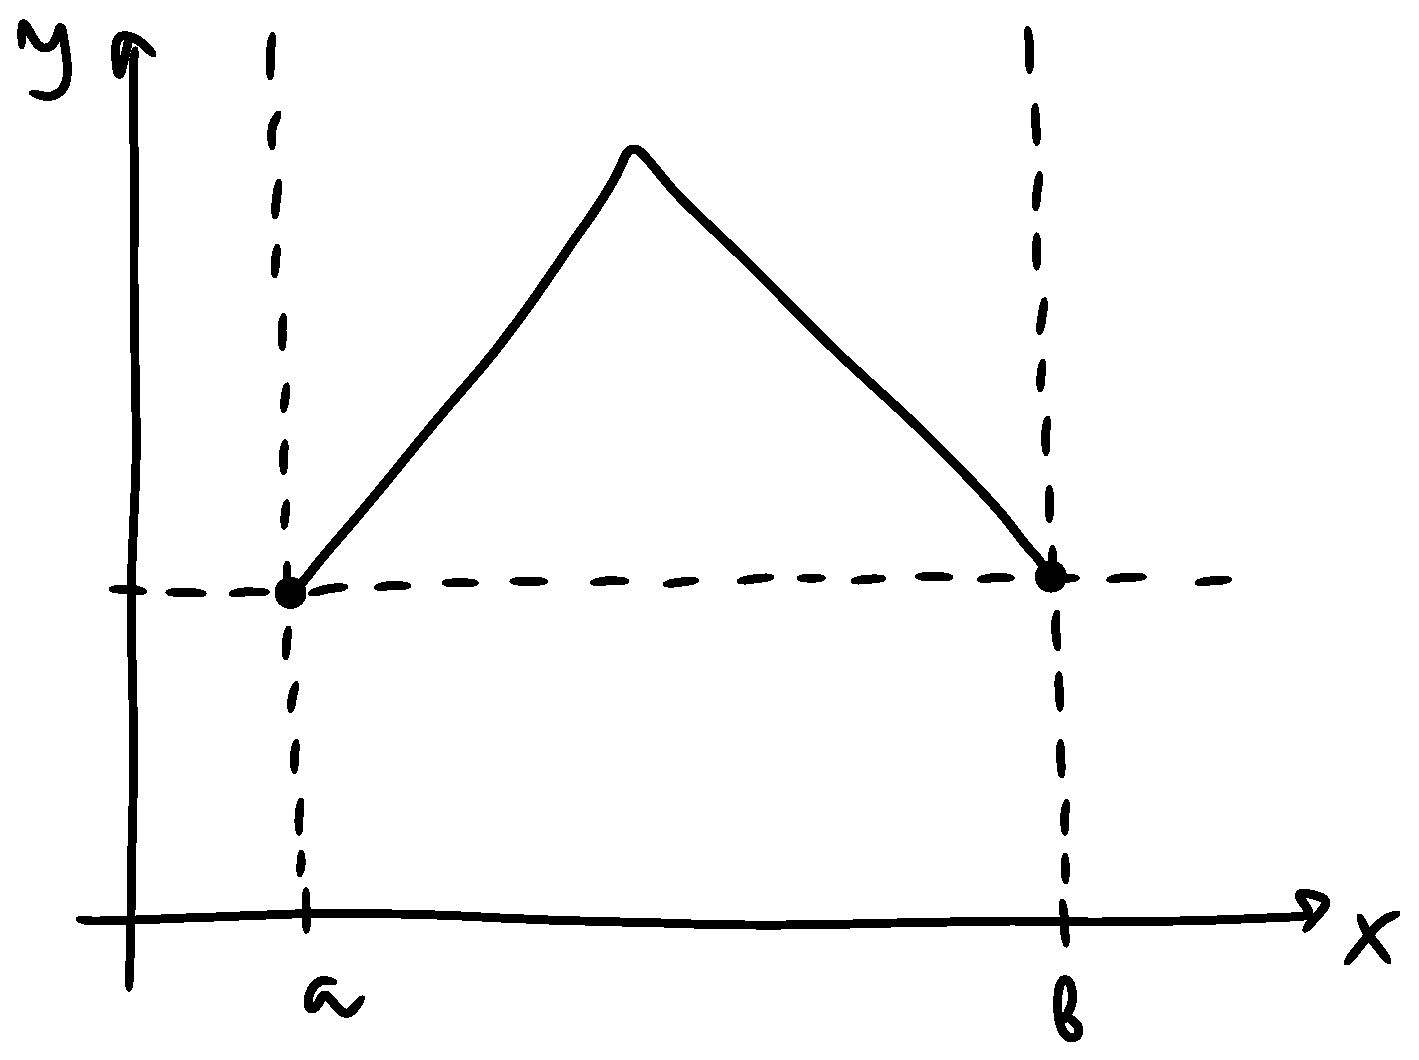
\includegraphics[width=\columnwidth]{images/not-roll-b}
        
        \caption{Без существования производной функции на интервале теорема Ролля может не работать.}
        \label{fig:1-16-33-b}
      \end{subfigure}
      %
      \hfill
      %
      \begin{subfigure}[b]{0.32\textwidth}
        \centering
        
        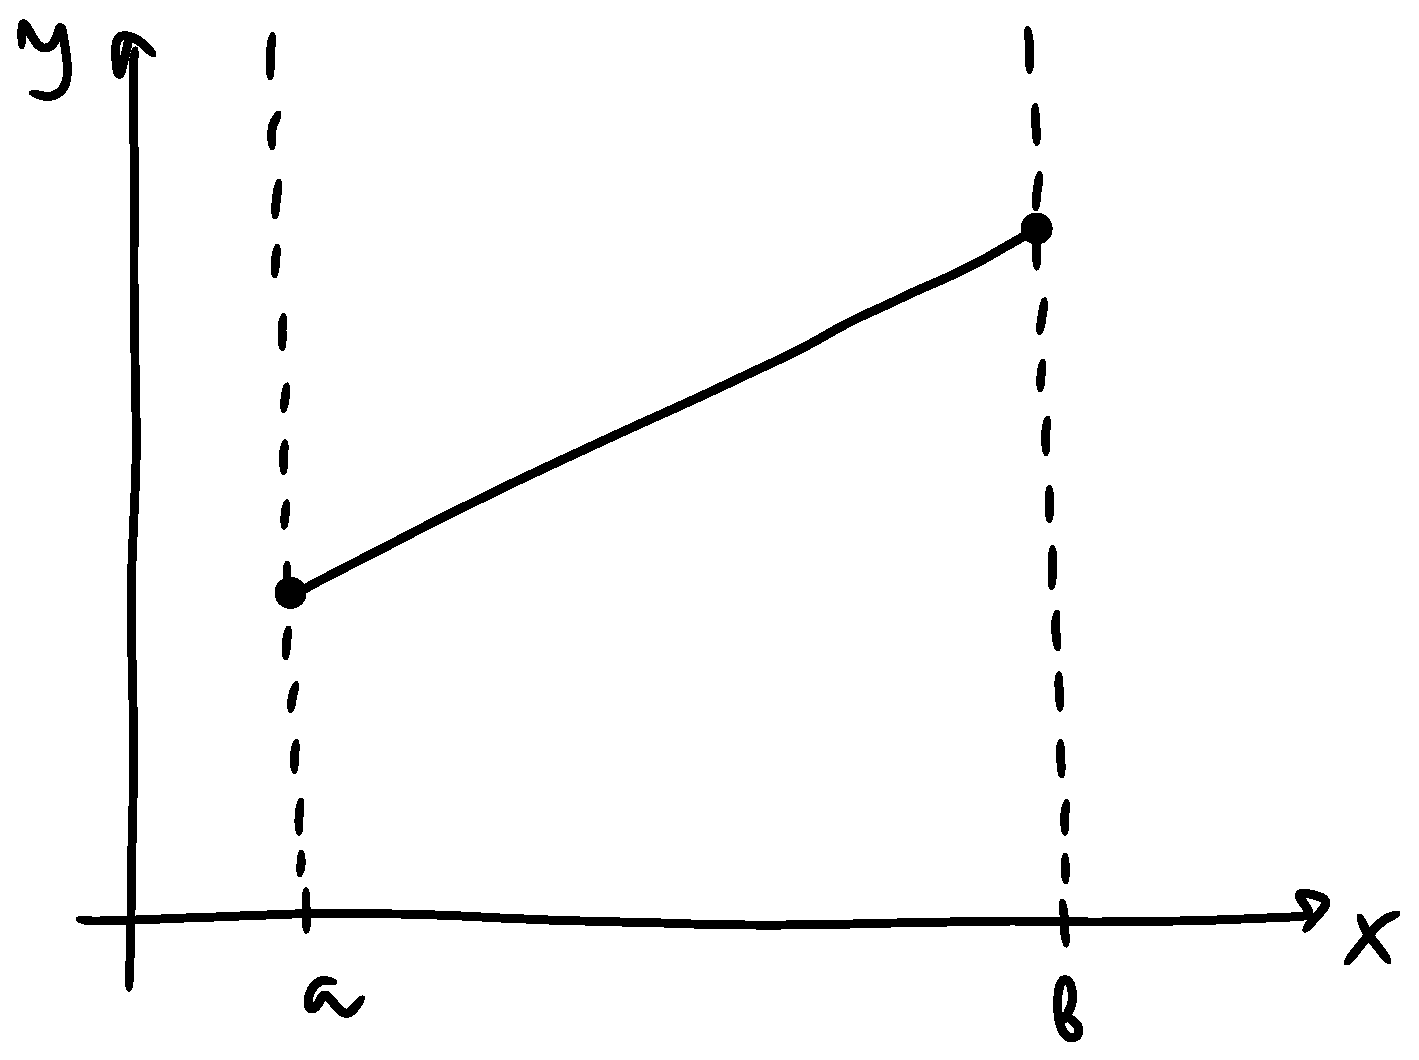
\includegraphics[width=\columnwidth]{images/not-roll-c}
        
        \caption{Без равенства значений функции на концах отрезка теорема Ролля может не работать.}
        \label{fig:1-16-33-c}
      \end{subfigure}
    \end{figure}
    % TODO: align images (captions)

    % \begin{figure}[ht]
    %     \centering
        
    %     \includegraphics[width=0.8\linewidth]{TODO}
        
    %     \caption{Без непрерывности функции на отрезке теорема Ролля может не работать.}
    %     \label{fig:1-16-33-a}
    % \end{figure}

    % \begin{figure}[ht]
    %     \centering
        
    %     \includegraphics[width=0.8\linewidth]{TODO}
        
    %     \caption{Без существования производной функции на интервале теорема Ролля может не работать.}
    %     \label{fig:1-16-33-b}
    % \end{figure}

    % \begin{figure}[ht]
    %     \centering
        
    %     \includegraphics[width=0.8\linewidth]{TODO}
        
    %     \caption{Без равенства значений функции на концах отрезке теорема Ролля может не работать.}
    %     \label{fig:1-16-33-c}
    % \end{figure}

  \end{solution}


  \subsection{С1, \S 16, \textnumero 30}

  Доказать, что если функция~$f$ дифференцируема на отрезке~$[1, 2]$, то существует такая точка~$\xi \hm\in (1, 2)$, что:
  \[
    f(2) - f(1) = \frac{\xi^2}{2} f'(\xi)
  \]
  
  \begin{solution}
    \mbox{}\par\noindent
    \emph{Эскиз решения}.
    
    На теорему Ролля не похоже, на Лагранжа тоже, поэтому...

    Перепишем доказываемое соотношение так, чтобы оно стало похоже хотя бы на ``третью теорему о среднем''~(\ref{theo:cochi}):
    \[
      f(2) - f(1) = \frac{f'(\xi)}{2/\xi^2}
    \]

    \emph{
      На этом ``эскиз'' заканчивается.
      Кажется, что сказанного достаточно, чтобы при желании довести решение до конца.
    }
  \end{solution}
  
  % \subsection{Приложение к теореме Лагранжа}\ref{appendix:lim-diff} % TODO: вместо гигантского footnote-а?

% \fi

\end{document}
